\documentclass[12pt]{article}
\usepackage[a4paper, total={7in,10in}]{geometry}
\usepackage{polyglossia}
\usepackage{ragged2e}
\usepackage{amsmath}
\usepackage{amssymb}
\usepackage{microtype}
\usepackage{graphicx}
\usepackage{changepage}
\graphicspath{{./images/}}
\setmainlanguage{russian}
\setotherlanguage{english}
\newfontfamily\russianfont[Script=Cyrillic]{Times New Roman}
\newfontfamily\englishfont{Times New Roman}
\setlength{\parindent}{0em}
\setlength{\parskip}{6pt}

\def\posl#1#2{\{#1_{#2}\}}

\begin{document}
    \justifying
    \tableofcontents
    \pagebreak
    \section{Введение}
    \subsection{Элементы теории множеств.}
    \subsubsection*{Определения (множества)}
    \noindent \underline{Множество} - совокупность объектов одинаковой природы.\\
    Обозначение: A, B, C - множества. a, b, c - элементы множества.\par
    \noindent Множества A и B называются равными, если они состоят из одних и тех же элементов.\\
    Множество A называется подмножеством множества B, если $\forall a \in A \implies a \in B$. Обозначение: $A \subset B$.\\
    Множество, не содержащее ни одного элемента, называется пустым множеством. Обозначение: $\varnothing$.\par
    \noindent Объединением множеств A и B ($A \cup B$) называется $C : C = \{ c : c \in A \cup c \in B \}$.\\
    Пересечением множеств A и B ($A \cap B$) называется $D : D = \{ d : d \in A \cap d \in B \}$.\\
    Разностью множеств A и B ($A \diagdown B$) называется $E : E = \{ e : e \in A \cap e \notin B \}$.\\
    Симметричной разностью множеств A и B ($A \triangle B$) называется $F : F = \{ f : f \in (A \diagdown B) \cup (B \diagdown A)\}$.
    \par
    \subsubsection*{Свойства операций}
    \begin{enumerate}
        \item $\forall A \text{ } A \subset A$\\$\forall A \text { } \varnothing \subset A$
        \item $A \cup A = A$\\$A \cap A = A$
        \item $A \cup \varnothing = A$\\$A \cap \varnothing = \varnothing$
        \item $A \subset B, B \subset C \implies A \subset C$
        \item $A \subset B, B \subset A \implies A = B$
        \item $A \diagdown (A \diagdown B) = A \cap B$
        \item $(A \cap B) \cup C = (A \cup C) \cap (B \cup C)$
        \item $(A \cup B) \cap C = (A \cap C) \cup (B \cap C)$
        \item $A \diagdown (B \cap C) = (A \diagdown B) \cup (A \diagdown C)$
        \item $A \diagdown (B \cup C) = (A \diagdown B) \cap (A \diagdown C)$
        \item $(A \diagdown B) \cup (B \diagdown A) = (A \cup B) \diagdown (A \cap B)$
    \end{enumerate}
    \par
    \subsubsection*{Доказательство пункта 9:}
    \begin{adjustwidth}{1.5em}{1.5em}
        Пусть X - произвольное множество.\\
        Если $x \in A \implies x \in A \cup X$\\
        Если $x \notin A \implies x \notin A \cap X$\\
        Если $x \in A \cap B \implies x \in A \text{ и } x \in B$\\
        Если $x \in A \cup B \implies x \in A \text{ или } x \in B$\\
        Если $x \notin A \cap B \implies x \notin A \text{ или } x \notin B$\\
        Если $x \notin A \cup B \implies x \notin A \text{ и } x \notin B$\\
        \\
        \text{а) Пусть }$x \in A \diagdown (B \cap C)$. Тогда $x \in A$ и $x \notin B \cap C$. Следовательно $x \in A$ и $(x \notin B)$ или $(x \notin C)$. Отсюда ($x \in A$ и $x \notin B$) или ($x \in A$ и $x \notin B$). Тогда $x \in (A \diagdown B) \cup (A \diagdown C)$.\\\\
        \text{б) Пусть }$x \in (A \diagdown B) \cup (A \diagdown C)$. Тогда $x \in (A \diagdown B)$ или $x \in (A \diagdown C)$. Пусть для определённости $x \in A \diagdown B$. Тогда $x \in A$ и $x \notin B$. Отсюда $x \in A$ и $x \notin B \cap X$, например $x \in A$ и $x \notin B \cap C \implies x \in A \diagdown (B \cap C)$.
        \begin{center}
            \textbf{Ч.т.д.}
        \end{center}
    \end{adjustwidth}
    \subsubsection*{Определения (декартово произведение)}
    \noindent Декартовым произведением множеств A и B ($A \times B$) называется множество $C : C = \{ (a; b) : a \in A \text{ и } b \in B\}$.\\
    Отображением F множества A в множество B называется подмножество их декартова произведения. $(F \subset A \times B) : \forall a \in A \text{ } \exists \text{ } ! \text{ } (a;b) \in F$.\\
    \underline{Примеры:}\par
    $A = \{1; 3; 5\}, B = \{2; 4; 6\}$
    \begin{itemize}
        \item $F = \{(1;2), (3;4), (5;6)\}$ - отображение
        \item $F = \{(1;2), (1;4), (3;4), (5;6)\}$ - не отображение
    \end{itemize}
    Пусть $F$ - отображение $A$ в $B$. Тогда элемент $b : (a;b) \in F$ называется образом элемента $a$ при отображении $F$. $b = F(a)$\\
    При этом $a$ называется прообразом (одним из возможных) элемента $b$.\\
    Множество $\{b \in B : \exists \text{ } a \in A : b = F(a)\}$ называется образом множества $A$ при отображении $F$ и обозначается $F(A)$.\par
    \noindent Отображение $F$ называется \textbf{сюръекцией} или отображением "на", если $F(A) = B$ (все элементы $b$ использованы в парах с элементами $a$)\\
    Отображение $F$ называется \textbf{инъекцией} или вложением, если $F(a_{1}) = F(a_{2}) \implies a_{1} = a_{2}$ (каждому элементу $a$ соответствует \underline{только один} элемент $b$)\\
    Отображение $F$ называется \textbf{биекцией} или взаимооднозначным отображением, если оно является и сюръекцией, и инъекцией.\par
    \noindent \underline{Пример:}  $A\{1;3;5\}, B\{2;4;6\}$
    \begin{itemize}
        \item $F_{1}\{(1;2),(3;2),(5;6)\}$ - не сюръекция, не инъекция.
        \item $F_{2}\{(1;2),(3;4),(5;6)\}$ - сюръекция, инъекция; следовательно, биекция.
    \end{itemize}

    \subsection{Мощность множества. Счётные и несчётные множества.}
    \subsubsection*{Эквивалентность}
    \noindent Множества $A$ и $B$ называются эквивалентными (равномощными), если между ними можно установить взаимооднозначное соответствие.\\
    Обозначение: $A \sim B$.\\
    \underline{Свойства:}
    \begin{enumerate}
        \item $A \sim A$ (свойство рефлексивности)
        \item $A \sim B \implies B \sim A$ (свойство симметричности)
        \item $A \sim B, B \sim C \implies A \sim C$ (свойство транзитивности)
    \end{enumerate}
    \subsubsection*{Мощность множеств. Счётные множества.}
    Множества чисел:
    \begin{itemize}
        \item $N$ - натуральные числа ($1;2;3;\dots$)
        \item $Z$ - целые числа ($0;\pm1;\pm2;\dots$)
        \item $Q$ - рациональные числа ($\frac{p}{q} : p \in Z, q \in N, \frac{p}{q}$ - несократимое)
        \item $R$ - действительные/вещественные числа
    \end{itemize}
    $N \subset Z \subset Q \subset R$\par
    \noindent \textbf{Мощность множества} - некая числовая характеристика (обозначающаяся $\#A$), обладающая свойствами:
    \begin{enumerate}
        \item Если $A$ - конечно, то $\#A$ - кол-во элементов множества.
        \item Если $A,B$ - бесконечномерные, то \begin{itemize}
            \item $\#A = \#B \Leftrightarrow A \sim B$
            \item $\#A \le \#B \Leftrightarrow A \sim C, C \subset B, \text{ но } A \text{ не} \subset B$
        \end{itemize}
    \end{enumerate}
    \underline{Утверждение:} $Z \sim N$\\
    \underline{Доказательство:}
    \begin{adjustwidth}{1.5em}{1.5em}
        $0;-1;1;-2;2;-3;3;\dots$\\
        $1;2;3;4;5;6;7;\dots$\\
        Каждому элементу $Z$ соответствует элемент $N$.        
    \end{adjustwidth}
    \noindent \underline{Утверждение:} $Q \sim N$\\
    \underline{Доказательство:}
        \begin{adjustwidth}{1.5em}{1.5em}
        Договоримся, что $0 = \frac{0}{1}$\\
        Обозначим $h = |p| + q$ - высота числа $\frac{p}{q}$\\
        Будем нумеровать рациональные числа по возрастанию $h$; при фиксированном $h$ - по возрастанию $q$; при фиксированном $h$ и $q$ - по возрастанию $p$.\\
        \begin{gather*}
            h = 1, q = 1 \implies p = 0 : r_{1} = \frac{0}{1}\\
            h = 2, q = 1 \implies p = \pm 1 : r_{2} = \frac{-1}{1}, r_{3} = \frac{1}{1}\\
            h = 2, q = 2 \implies p = 0 \text{ (не может быть по определению)}\\
            h = 3, q = 1 \implies p = \pm 2 : r_{4} = \frac{-2}{1}, r_{5} = \frac{2}{1}\\
            h = 3, q = 2 \implies p = \pm 1 : r_{6} = \frac{-1}{2}, r_{7} = \frac{1}{2}\\
            h = 3, q = 3 \implies p = 0 \text{ (не может быть по определению)}\\
        \end{gather*}
        Индексы $r$ являются натуральными числами $\implies$ каждому рациональному числу можно поставить в соответствие натуральное число.
        \end{adjustwidth}
    \begin{center}
        \textbf{Ч.т.д.}
    \end{center}
    Множества, эквивалентные множеству $N$, называются \underline{счётными}.\\\\
    \underline{Утверждение:} $\forall$ непустое подмножество счётного множества конечно или счётно.\\
    \underline{Доказательство:} занумеруем все элементы множества, затем перенумируем элементы подмножества в порядке возрастания номеров. Либо элементы закончатся, либо получим счётное подмножество.
    \begin{center}
        \textbf{Ч.т.д.}
    \end{center}
    \par
    \noindent \underline{Утверждение:} счётное объединение счётных множеств счётно.\\
    \underline{Доказательство:}
    \begin{gather*}
        A_{1} = \{a_{11}; a_{12}; \dots; a_{1n}\} \text{- счётное}\\
        A_{2} = \{a_{21}; a_{22}; \dots; a_{2n}\} \text{- счётное}\\
        A_{3} = \{a_{31}; a_{32}; \dots; a_{3n}\} \text{- счётное}\\
        A = \{a_{11}; a_{21}; a_{12}; a_{13}; a_{22}; a_{31}; a_{32}; \dots\}\\
        N = \{1; 2; 3; 4; 5; 6; 7; \dots\}
    \end{gather*}
    \begin{adjustwidth}{1.5em}{1.5em}
        Каждому элементу множества $A$ можно поставить в соответствие натуральное число из множества $N$. 
        \begin{center}
            \textbf{Ч.т.д.}
        \end{center}
    \end{adjustwidth}
    \subsubsection*{Несчётные множества.}
    \subsubsection*{Теорема 2.1:} 
    Множество $H$ всех бесконечных наборов из цифр $0$ и $1$ не является счётным.\par
    \noindent \underline{Доказательство:}
    \begin{adjustwidth}{1.5em}{1.5em}
        Пусть $h \in H, h = (h_{1}, h_{2}, h_{3}, \dots, h_{k}, \dots,), h_{k} = 0 \text{ или } 1$\\
        Предположим противное. Пусть $H$ - счётное, т.е. $H = \{h^{1},h^{2},h^{3},\dots,h^{j},\dots,h^{k},\dots\}$
        \[
            h^{1} = \{h_{1}^{1}, h_{2}^{1}, h_{3}^{1},\dots,\dots\}
        \]
        \[
            h^{2} = \{h_{1}^{2}, h_{2}^{2}, h_{3}^{2},\dots,\dots\}
        \]
        \[\vdots\]
        \[
            h^{j} = \{h_{1}^{j}, h_{2}^{j}, \dots, h_{j}^{j},\dots\}
        \]
        \[\vdots\]
        \[
            h^n = \{h_{1}^n, h_{2}^n,\dots, h_{n}^n,\dots\}
        \]
        Построим набор $\bar{h} = \{\bar{h_{1}^{1}};\bar{h_{2}^{2}};\dots;\bar{h_{j}^{j}};\dots;\bar{h_{n}^n};\dots\}$, где $\bar{h_{k}^{k}} = \begin{cases}0,\text{если } h_{k}^{k} = 1\\1,\text{если } h_{k}^{k} = 0\end{cases}$
        Очевидно, что $\bar{h} \in H$, т.е. $\bar{h}$ имеет номер, пусть $\bar{h} = h^{j}$\\
        На $j$-ом месте $h^{j}$ имеет элемент $h^{j}_{j}$\\
        На $j$-ом месте $\bar{h}$ имеет элемент $\bar{h^{j}_{j}}$, т.е. $h^{j}_{j} = \bar{h^{j}_{j}}$\\
        Получили противоречие. Таким образом $H$ не является счётным.
        \begin{center}
            \textbf{Ч.т.д.}
        \end{center}    
    \end{adjustwidth}
    \textbf{Следствие:} множество всех подмножеств счётного множества не является счётным.
    \subsubsection*{Теорема 2.2:}
    Множество $K$ всех бесконечных наборов, состоящих из цифр от 0 до 9, не является счётным.\par\noindent
    \underline{Доказательство:} очевидно, что $H \subset K$. Если бы $K$ было счётным, то и $H$ было бы счётным, а это не так.
    \begin{center}
        \textbf{Ч.т.д.}
    \end{center}
    Множества, эквивалентные множеству вещественных чисел отрезка $[0;1]$ называются множествами мощности континуума.

    \subsection{Понятие рационального числа. Понятие вещественного числа.}
    \noindent Рациональными числами будем называть числа вида \[\frac{p}{q}, p \in Z, q \in N, \text{НОД}(p,q) = 1, 0 = \frac{0}{1}\]
    Множество рациональных чисел - $Q$.
    \subsubsection*{Свойства:}
    \begin{enumerate}
        \item $\forall a,b \in Q$ $|$ $a < b$ или $a = b$ (правило упорядочивания)
        \item $\forall a,b \in Q$ $\exists!$ $c \in Q$ $|$ $ c = a + b$ (корректность определения суммы)
        \item $\forall a,b \in Q$ $\exists!$ $d \in Q$ $|$ $ d = ab$ (корректность определения произведения)
        \item $\forall a,b,c \in Q$ если $a < b$, а $b < c \implies a < c$\\$\forall a,b,c \in Q$ если $a = b$, а $b = c \implies a = c$ (транзитивность)
        \item $\forall a,b \in Q$ $|$ $a+b=b+a$ (коммутативность сложения)
        \item $\forall a,b,c \in Q$ $|$ $(a+b)+c = a+(b+c)$ (ассоциативность сложения)
        \item $\exists!$ $0 \in Q$ $|$ $\forall a \in Q$ $a+0 = 0+a = a$ (существование нейтрального элемента по сложению)
        \item $\forall a \in Q$ $\exists!$ $a' \in Q$ $|$ $a+a'=a'+a = 0$ (существование обратного элемента по сложению)
        \item $\forall a,b \in Q$ $|$ $ab=ba$ (коммутативность умножения)
        \item $\forall a,b,c \in Q$ $|$ $(ab)c = a(bc)$ (ассоциативность умножения)
        \item $\exists!$ $1 \in Q$ $|$ $\forall a \in Q$ $a \times 1 = 1 \times a = a$ (существование нейтрального элемента по умножению)
        \item $\forall a \ne 0, a \in Q$ $\exists!$ $a' \in Q$ $|$ $a \times a'=a' \times a = 1$ (существование обратного элемента по умножению)
        \item $\forall a,b,c \in Q$ $(a + b)c = ac + bc$ (дистрибутивность)
        \item если $a < b, c \in Q \implies a+c < b+c$
        \item если $a < b, c > 0 \implies ac < bc$
        \item $\forall a \in Q$ $\exists$ $n \in N$ $|$ $n > a$ (аксиома Архимеда, или "натуральных чисел бесконечно много")
    \end{enumerate}
    \subsubsection*{Вещественные числа}
    \noindent Вещественным или действительным числом называется произвольная бесконечная десятичная дробь вида $\pm a_{1},a_{2}a_{3}a_{4}\dots a_{n} \dots$\\
    Рассмотрим $0,(9) = 0,9999\dots \in Q$\\
    \[0,(9) = \frac{9}{10} + \frac{9}{100} + \frac{9}{1000} + \dots = \begin{vmatrix}
        S & = & \frac{b_{1}}{1-q}\\
        b_{1} & = & \frac{9}{10}\\
        q & = & \frac{1}{10}
    \end{vmatrix} = \frac{\frac{9}{10}}{1-\frac{1}{10}} = 1\]\\
    Договоримся, что рациональное число не может содержать в своей записи бесконечное число 9.\\
    Модуль (абсолютная величина) числа $a = \pm a_{0},a_{1}a_{2}\dots a_{n}\dots$ называется число, выраженное той же дробью, что и $a$, но взятой со знаком "+".
    \subsubsection*{Правила сравнения вещественных чисел}
    \begin{enumerate}
        \item Пусть $a = \pm a_{0},a_{1}a_{2}\dots a_{n}\dots$\\
        $b = \pm b_{0},b_{1}b_{2}\dots b_{n}\dots$\\
        $a,b \in R$\\
        Числа $a$ и $b$ называются равными, если перед ними один знак и $a_{0} = b_{0}, a_{1} = b_{1}, \dots, a_{n} = b_{n}, \dots$
        \item Пусть $a \ne b$
        \begin{itemize}
            \item $\forall$ положительное число $> 0$
            \item $\forall$ отрицательное число $< 0$
            \item $\forall$ положительное число $>$ $\forall$ отрицательного числа
            \item $a > 0, b > 0$. Будем говорить, что $a > b$, если $a_{0}=b_{0}, a_{1}=b_{1},\dots,a_{k}>b_{k}$.
            \item $a < 0, b < 0$. $a > b$, если $|a| < |b|$; $a < b$, если $|a| > |b|$.
        \end{itemize}
    \end{enumerate}

    \subsection{Ограниченные множества вещественных чисел.}
    \subsubsection*{Ограниченные множества}
    \noindent Множество $X \subset R$ ограничено сверху, если $\exists$ $M \in R$ $|$ $\forall x \in X$ $x \le M$\\
    Множество $X \subset R$ ограничено снизу, если $\exists$ $m \in R$ $|$ $\forall x \in X$ $x \ge m$\\
    Числа $M$ и $m$ называются верхней и нижней гранями множества $X$ соответственно.\\
    Число $\bar{x} \in R$ ($\underline{x} \in R$) называется точной верхней (нижней) гранью множества $X$, если:
    \begin{enumerate}
        \item $\forall x \in X$ $x \le \bar{x}$ $(x \ge \underline{x})$
        \item $\forall x' \in R$ $|$ $x' < \bar{x}$ $\exists$ $x_{0} \in X$ $|$ $x_{0} > x'$ ($\forall x' \in R$ $|$ $x' > \underline{x}$, $\exists$ $x_{0} \in X$ $x_{0} < x'$) (невозможность уменьшить точную грань)
        \item (на самом деле 2*): $\forall \varepsilon > 0$ $\exists$ $N = N(\varepsilon)$ $|$ $\bar{x} - \varepsilon < x_n$\\
        $\forall \varepsilon > 0$ $\exists$ $N = N(\varepsilon)$ $|$ $\underline{x} - \varepsilon > x_n$
    \end{enumerate} 
    Обозначения:
    \begin{itemize}
        \item $\bar{x} = \sup x$ - супремум множества X
        \item $\underline{x} = \inf x$ - инфинум множества X
    \end{itemize}
    \subsubsection*{Теорема 4.1 (принцип полноты Вейерштрасса):}
    $\forall$ непустое ограниченное сверху (снизу) множество $X \subset R$ имеет точную верхнюю (нижнюю) грань.

    \subsection{Арифметические операции над вещественными числами. Свойства вещественных чисел.}
    \subsubsection*{Леммы}
    \noindent \textbf{Лемма 1:} пусть $a \in R$\\
    $\forall \varepsilon > 0, \varepsilon \in Q$ $\exists$ $\alpha, \beta \in Q$ $|$ $\alpha \le a \le \beta,$ причём $\beta - \alpha < \varepsilon$\\\\
    \underline{Доказательство:}
    \begin{adjustwidth}{1.5em}{1.5em}
        Пусть $a = a_{0},a_{1}a_{2}a_{3}\dots a_{n}\dots \ge 0$\\
        Пусть $\alpha = a_{0},a_{1}a_{2}a_{3}\dots a_{n}.$ Очевидно, что $\alpha \le a$.\\
        Положим $\beta = \alpha + \frac{1}{10^n}$\\
        $\beta = a_{0},a_{1}a_{2}a_{3}\dots (a_{n}+1)$. Очевидно, что $\beta \ge a$\\
        \underline{Замечание:} \[\forall \varepsilon > 0, \varepsilon \in Q \text{ } \exists \text{ } n \in N \implies | \text{ } 10^n > \frac{1}{\varepsilon} \text{ (аксиома Архимеда)}\]
        \[\beta - \alpha = \frac{1}{10^n} < \varepsilon\].
        \begin{center}
            \textbf{Ч.т.д.}
        \end{center}    
    \end{adjustwidth}

    \noindent \textbf{Лемма 2:} $\forall a,b \in R$ $\exists$ $\alpha \in Q$ $|$ $a < \alpha < b$\\
    \underline{Замечание:} таких $\alpha$ бесконечно много.\\\\
    \underline{Доказательство:} 
    \begin{adjustwidth}{1.5em}{1.5em}
        Пусть $a = a_{0},a_{1}\dots a_{n}\dots \ge 0$\\
        Пусть $a = a_{0},a_{1}\dots a_{k}99\dots9a_{p}\dots$ при $a_{p} \ne 9$\\
        $b = b_{0},b_{1}\dots b_{k}\dots$, $a_{0}=b_{0}, a_{1} = b_{1}, \dots, a_{k} < b_{k} \implies a < b$\\
        $\alpha = a_{0},a_{1}\dots a_{k}99\dots9(a_{p}+1)$.\\
        $a < \alpha$, т.к. $a_{p} < a_{p} + 1$\\
        $b > \alpha$, т.к. $a_{k} < b_{k}$\\
        Следовательно $a < \alpha < b$\\
        Если $a < 0$, $b > 0$, то $\alpha = 0,000\dots$\\
        Если $a < b \le 0$, то переходим к модулям.
        \begin{center}
            \textbf{Ч.т.д.}
        \end{center}
    \end{adjustwidth}

    \noindent \textbf{Лемма 3:} пусть $a,b \in R$. Если $\forall \varepsilon > 0, \varepsilon \in Q$ $|$ $\exists$ $\gamma_{1}, \gamma_{2} \in Q$ $|$ $\gamma_{1} \le a \le \gamma_{2}$ и $\gamma_{1} \le b \le \gamma_{2}$ и $\gamma_{1} - \gamma_{2} < \varepsilon$, то $a = b$.\\\\
    \underline{Доказательство:} 
    \begin{adjustwidth}{1.5em}{1.5em}
        Предположим противное.\\
        Пусть $a \ne b$; пусть для определённости $a < b$. Тогда по лемме 2 $\exists$ $\alpha_{1}, \alpha_{2} \in Q$ $|$ $a < \alpha_{1} < \alpha_{2} < b$\\
        Положим $\varepsilon = \frac{\alpha_{2}-\alpha_{1}}{2}$. По условию леммы $\exists$ $\gamma_{1}, \gamma_{2} \in Q$ $|$ $\gamma_{1} \le a < \alpha_{1} < \alpha_{2} < b \le \gamma_{2}$ и $\gamma_{2} - \gamma_{1} < \varepsilon$\\
        Отсюда $\gamma_{1} < \alpha_{1} < \alpha_{2} < \gamma_{2}$. Отнимем $\gamma_{1}$.\\
        \[0 < \alpha_{2} - \alpha_{1} < \alpha_{2}-\gamma_{1} < \gamma_{2}-\gamma_{1}\]
        \[\alpha_{2} - \alpha_{1} > \varepsilon, \gamma_{2} - \gamma_{1} < \varepsilon\]
        Получили противоречие. Следовательно, $a = b$.
        \begin{center}
            \textbf{Ч.т.д.}
        \end{center}
    \end{adjustwidth}

    \subsubsection*{Арифметические действия}
    \noindent Суммой чисел $a,b \in R$ называется число $c \in R$ $|$ $\forall \alpha_{1}, \alpha_{2}, \beta_{1}, \beta_{2} \in Q; \alpha_{1} \le a \le \alpha_{2}; \beta_{1} \le b \le \beta_{2}$ выполнено $\alpha_{1} + \beta_{1} \le c \le \alpha_{2} + \beta_{2}$\par\noindent
    \noindent Произведением чисел $a,b \in R$ называется число $c \in R$ $|$ $\forall \alpha_{1}, \alpha_{2}, \beta_{1}, \beta_{2} \in Q; \alpha_{1} \le a \le \alpha_{2}; \beta_{1} \le b \le \beta_{2}$ выполнено $\alpha_{1}\beta_{1}\le c \le \alpha_{2}\beta_{2}$\par\noindent
    \underline{Замечание:} все операции с вещественными числами производятся с погрешностью.\\\\
    По определению положим: $a \times 0 = 0 \times a = 0$\\
    Пусть $a,b \in R$. Тогда по определению
    \[ab = \begin{cases}
        |a||b|\text{, если }ab > 0\text{ (a и b одного знака)}\\
        -|a||b|\text{, если }ab < 0\text{ (a и b разных знаков)}
    \end{cases}\]
    \subsubsection*{Свойства вещественных чисел}
    \begin{enumerate}
        \item $\forall a,b \in R$ $|$ $a < b$ или $a = b$ (правило упорядочивания)
        \item $\forall a,b \in R$ $\exists!$ $c \in R$ $|$ $ c = a + b$ (корректность определения суммы)
        \item $\forall a,b \in R$ $\exists!$ $d \in R$ $|$ $ d = ab$ (корректность определения произведения)
        \item $\forall a,b,c \in R$ если $a < b$, а $b < c \implies a < c$\\$\forall a,b,c \in R$ если $a = b$, а $b = c \implies a = c$ (транзитивность)
        \item $\forall a,b \in R$ $|$ $a+b=b+a$ (коммутативность сложения)
        \item $\forall a,b,c \in R$ $|$ $(a+b)+c = a+(b+c)$ (ассоциативность сложения)
        \item $\exists!$ $0 \in R$ $|$ $\forall a \in R$ $a+0 = 0+a = a$ (существование нейтрального элемента по сложению)
        \item $\forall a \in R$ $\exists!$ $a' \in R$ $|$ $a+a'=a'+a = 0$ (существование обратного элемента по сложению)
        \item $\forall a,b \in R$ $|$ $ab=ba$ (коммутативность умножения)
        \item $\forall a,b,c \in R$ $|$ $(ab)c = a(bc)$ (ассоциативность умножения)
        \item $\exists!$ $1 \in R$ $|$ $\forall a \in R$ $a \times 1 = 1 \times a = a$ (существование нейтрального элемента по умножению)
        \item $\forall a \ne 0, a \in R$ $\exists!$ $a' \in R$ $|$ $a \times a'=a' \times a = 1$ (существование обратного элемента по умножению)
        \item $\forall a,b,c \in R$ $(a + b)c = ac + bc$ (дистрибутивность)
        \item если $a < b, c \in Q \implies a+c < b+c$
        \item если $a < b, c > 0 \implies ac < bc$
        \item $\forall a \in R$ $\exists$ $n \in N$ $|$ $n > a$ (аксиома Архимеда, или "натуральных чисел бесконечно много")
    \end{enumerate}
    \subsubsection*{Арифметические действия 2. Electric Boogalo}
    \noindent Разностью чисел $a,b \in R$ называется число $c \in R$ $|$ $a = c+b$\\
    Покажем, что этому определению удовлетворяет число $c = a + b'$, где $b'$ - обратное к $b$ по сложению.\\
    Действительно $c + b = (a + b') + b = a + (b' + b) = a + 0 = a$\\
    Покажем, что $c$ - единственное.\\
    Пусть $\exists$ $d \in R$ $|$ $a = d + b$, тогда $c = a + b' = d + b + b' = d + 0 = d$\\
    Т.е. разность определена единственным образом.\\
    По определению $0-b = 0+b' = b' = -b$\\
    Пишем, что $b' = 0 - b = -b$\\
    Обозначение: $c = a - b$\par\noindent
    Частным чисел $a,b \in R, b \ne 0$ называется число $c \in R$ $|$ $a = bc$\\
    Покажем, что этому определению удовлетворяет число $c = ab'$, где $b'$ - обратное к $b$ по умножению.\\
    Действительно $cb = (ab')b = a(b'b) = a \times 1 = a$\\
    Покажем, что $c$ - единственное.\\
    Пусть $\exists$ $d \in R$ $|$ $a = db$, тогда $c = ab' = (db)b' = d(bb') = d$\\
    Т.е. частное определено единственным образом.\\
    Обозначение: $c = \frac{a}{b}$

    \section{Теория пределов числовых последовательностей.}

    \subsection{Числовая последовательность. Предел числовой последовательности.}
    \subsubsection*{Определение числовой последовательности.}
    \noindent Пусть каждому натуральному $n \in N$ по определённому закону ставится в соответствие действительное число $x_n$.\\
    Тогда говорят, что определена \underline{числовая последовательность}.\\
    Обозначение: $\{x_n\}$\\
    $x_{1}, x_{2}, \dots, x_n, \dots$ - элементы последовательности.\\
    \underline{Пример:} арифметическая прогрессия $x_n = a + d(n-1)$, геометрическая прогрессия $x_n = a \times q^n$.\par\noindent
    При $a < b$:
    \begin{itemize}
        \item Множество чисел $x$ $|$ $a \le x \le b$ называется отрезком $[a; b]$
        \item Множество чисел $x$ $|$ $a < x < b$ называетя интервалом $(a; b)$
        \item Если $a \le x < b$ или $a < x \le b$, то есть $[a; b)$ или $(a; b]$, то эти множества называются полуинтервалом или полуотрезком.
        \item \underline{Замечание:} $a, b$ могут быть $\infty$ и $-\infty$ и образовывать, например, $(-\infty; \infty), [a, \infty)$ и т.д.
    \end{itemize}
    Произвольный интервал $(a; b)$, содержащий точку $c$ $(a < c < b)$ называется окрестностью точки $c$ и обозначается $U(c)$.
    \subsubsection*{Крайне важные определения}
    \noindent Интервал вида $(c - \varepsilon; c + \varepsilon)$ при $\varepsilon > 0$ называется $\varepsilon$-окрестностью точки $c$.\par\noindent
    Число $a$ называется \textbf{пределом} числовой последовательности $x_n$, если 
    \[\forall \varepsilon > 0 \text{ } \exists \text{ } N = N(\varepsilon) \text{ } \big| \text{ } \forall n > N \implies |x_n - a| < \varepsilon\]
    Говоря по-русски, для любого эпсилон больше нуля существует номер $N$, зависящий от эпсилон, при котором при любом номере $n$ больше номера $N$ выполняется неравенство: $|x_n - a|$ меньше эпсилон.\\
    Есть такие последовательности, чьих пределов не существует, например, \[\lim_{n\to\infty}(-1)^n = \nexists\]
    \underline{Пример:} $x_n = \frac{1}{n}$. Докажем, что $\lim_{n\to\infty}x_n = 0$.
    \begin{gather*}
        |\frac{1}{n} - 0| < \varepsilon\\
        \frac{1}{n} < \varepsilon\\
        1 < n\varepsilon\\
        n > \frac{1}{\varepsilon}\\
        N(\varepsilon) = [\frac{1}{\varepsilon}]\\
    \end{gather*}
    \begin{gather*}
        \textbf{Проверка:}\\
        \varepsilon = \frac{1}{10}\\
        N(0.1) = 10\\
        x_{10} = \frac{1}{10} \notin \varepsilon\text{-окр.}\\
        x_{11} = \frac{1}{11} \in \varepsilon\text{-окр.}\\\\ 
        \varepsilon = \frac{1}{100}\\
        N(0.01) = 100\\
        x_{100} = \frac{1}{100} \notin \varepsilon\text{-окр.}\\
        x_{101} = \frac{1}{101} \in \varepsilon\text{-окр.}\\\\
        \textbf{Ч.т.д.}
    \end{gather*}

    \noindent Последовательность, имеющая конечный предел, называется сходящейся последовательностью.\\В противном случае - расходящейся.

    \subsection{Теоремы о сходящихся последовательностях}
    \subsubsection*{Теорема 2.1:}
    Если $\posl{x}{n}$ имеет предел, то он единственный.\par\noindent
    \underline{Доказательство:}
    \begin{adjustwidth}{1.5em}{1.5em}
        Предположим противное. Пусть $\lim_{n\to\infty}x_n = a, \lim_{n\to\infty}x_n = b, a \ne b$, пусть для определённости $a < b$.\\
        Выберем окрестности точки $a$ и $b$ таким образом, чтобы они не пересекались.\\
        %\includegraphics{2.2.1}\\
        По условию $\lim_{n\to\infty} x_n = a \implies$ в окрестность точки $a$ попадает $\infty$-ое число элементов $\posl{x}{n}$\\
        Вне этой окрестности находится конечное число элементов $\posl{x}{n}$ $\implies$ в окрестность точки $b$ попадает конечное число элементов $\posl{x}{n}$.\\
        Получили противоречие, т.к. $\lim_{n\to\infty}x_n = b \implies$ в окрестности точки $b$ должно быть $\infty$-ое число элементов $\posl{x}{n}$.\\
        Отсюда следует, что $a = b$.
        \begin{center}
            \textbf{Ч.т.д.}
        \end{center}    
    \end{adjustwidth}
    \subsubsection*{Теорема 2.2:}
    Если $\posl{x}{n}$ сходится, то она ограничена.\par\noindent
    \underline{Доказательство:}
    \begin{adjustwidth}{1.5em}{1.5em}
        Пусть $\posl{x}{n}$ сходится. Тогда существует конечный $\lim_{n\to\infty}x_n = a$, т.е.
        \[
            \forall \varepsilon > 0 \text{ } \exists \text{ } N = N(\varepsilon) \text{ } \big| \text{ } \forall n > N \implies |x_n - a| < \varepsilon
        \]
        Рассмотрим $|x_{1} - a| \ge \varepsilon, |x_{2} - a| \ge \varepsilon, \dots, |x_n - a| \ge \varepsilon$\\
        Обозначим $max\{|x_{1} - a|, |x_{2} - a|, \dots, |x_n - a|\} = d \implies d \ge \varepsilon$\\
        Тогда
        \[
            \begin{cases}
                \forall n = 1..N \implies |x_n - a| \le d\\
                \forall n > N \implies |x_n - a| < \varepsilon \le d
            \end{cases}
            \implies
            \forall N \implies |x_n - a| \le d
        \]
        \[
            a - d \le x_n \le a + d
        \]
        Отсюда следует, что $\posl{x}{n}$ ограничена.\\
        \begin{center}
            \textbf{Ч.т.д.}
        \end{center}
    \end{adjustwidth}
    
    \noindent \underline{Замечание:} ограниченность подпоследовательности является необходимым условием, но не является достаточным, т.е. если $\posl{x}{n}$ ограничена, то она не обязана сходиться.\\
    Пример:
    \[
        \posl{x}{n} = (-1)^n \Rightarrow -1; 1; -1; 1; \dots
    \]
    $\posl{x}{n}$ ограничена, но $\lim_{n\to\infty}x_n = \nexists$\\
    У данной последовательности нет такого элемента, который если окружить окрестностью ("ловушкой"), получится "поймать" все элементы последовательности.
    \subsubsection*{Теорема 2.3 (о сохранении знака):}
    \begin{adjustwidth}{1.5em}{1.5em}
        Если $\lim_{n\to\infty}x_n = a \ne 0$, то $\exists \text{ } N = N(\varepsilon) \text{ } \big| \text{ } \forall n > N \implies |x_n| > \frac{a}{2}$\\
        Если $a > 0$, то $x_n > \frac{a}{2}$\\
        Если $a < 0$, то $x_n < \frac{a}{2}$    
    \end{adjustwidth}
    \underline{Доказательство:} 
    \begin{adjustwidth}{1.5em}{1.5em}
        Пусть $\lim_{n\to\infty} x_n = a$. Зафиксируем $\varepsilon = \frac{|a|}{2}$.
    \end{adjustwidth}
    \begin{gather*}
        \forall \varepsilon > 0 \text{ } \exists \text{ } N = N(\varepsilon) \text{ } \big| \text{ } \forall n > N \implies |x_n - a| < \varepsilon\\
        a - \frac{|a|}{2} < x_n < a + \frac{|a|}{2}
    \end{gather*}
    \begin{align*}
        &\textbf{a > 0} & &\textbf{a < 0}\\
        x_n &> a - \frac{|a|}{2} & x_n &< a + \frac{|a|}{2}\\
        x_n &> \frac{a}{2} & x_n &< \frac{a}{2}
    \end{align*}
    \begin{center}
        \textbf{Ч.т.д.}
    \end{center}
    \subsubsection*{Теорема 2.4:}
    Если $\lim_{n\to\infty}x_n = a, \lim_{n\to\infty}y_n = b$ и $\forall n \in N$ $x_n \le y_n$, то $a \le b$.\par\noindent
    \underline{Доказательство:} 
    \begin{adjustwidth}{1.5em}{1.5em}
        Предположим противное.\\
        Пусть $a > b$. Зафиксируем $\varepsilon = \frac{a-b}{2}$.\\
        Т.к. $\lim_{n\to\infty} x_n = a$, то для $\varepsilon = \frac{a-b}{2}$ $\exists N_{1}$ $\big|$ $\forall n > N_{1}$ $|x_n - a| < \varepsilon$
        \[
            a - \varepsilon < x_n < a + \varepsilon
        \]
        Т.к. $\lim_{n\to\infty} y_n = b$, то для $\varepsilon = \frac{a-b}{2}$ $\exists N_{2}$ $\big|$ $\forall n > N_{2}$ $|y_n - b| < \varepsilon$
        \[
            b - \varepsilon < y_n < b + \varepsilon
        \]
        Пусть $N = max\{N_{1}, N_{2}\}$. Тогда $\forall n > N$
        \begin{gather*}
            y_n < b + \varepsilon = b + \frac{a-b}{2} = \frac{a}{2} + \frac{b}{2} =\\
            \frac{a}{2} + \frac{b}{2} + \frac{a}{2} - \frac{a}{2} = a - \frac{a-b}{2} = a - \varepsilon < x_n\\
            y_n < x_n
        \end{gather*}
        Получили противоречие. Таким образом, $a \le b$.
        \begin{center}
            \textbf{Ч.т.д.}
        \end{center}        
    \end{adjustwidth}
    
    \noindent \textbf{Следствие:} если $\posl{x}{n}$ - сходящаяся подпоследовательность и $\forall n \in N$ $x_n \in [a;b]$, то её предел $\in [a;b]$\\
    \underline{Доказательство:} 
    \begin{adjustwidth}{1.5em}{1.5em}
        $\forall n$ $a_{n} \le x_n \le b_{n}$\\
        Пусть $\lim_{n\to\infty}x_n = c$.\\
        Рассмотрим $\posl{a}{n}$. Её элементы: $a; a; a; a; \dots$\\
        $\lim_{n\to\infty}a_{n} = a$\\
        $\forall n$ $a_{n} \le x_n \implies a \le c$ (по теореме 2.4).\\
        Аналогично $c \le b$. Следовательно, $a \le c \le b$.
        \begin{center}
            \textbf{Ч.т.д.}
        \end{center}
    \end{adjustwidth}

    \subsubsection*{Теорема 2.5 ("теорема о двух милиционерах"):}
    Если $\lim_{n\to\infty} x_n = a, \lim_{n\to\infty} y_n = a$ и $\forall n \in N$ $x_n \le z_{n} \le y_n$, то $\lim_{n\to\infty} z_{n} = a$\par\noindent
    \underline{Доказательство:}
    \begin{adjustwidth}{1.5em}{1.5em}
        Зафиксируем $\varepsilon$.\\
        \[\lim_{n\to\infty} x_n = a \implies \exists N_{1} \text{ } \big| \text{ } \forall n > N_{1} \text{ } a-\varepsilon < x_n < a + \varepsilon\]
        \[\lim_{n\to\infty} y_n = a \implies \exists N_{2} \text{ } \big| \text{ } \forall n > N_{2} \text{ } a-\varepsilon < y_n < a + \varepsilon\]
        Пусть $N = max\{N_{1}, N_{2}\}$. Тогда $\forall n > N$
        \[a-\varepsilon < x_n \le z_{n} \le y_n < a + \varepsilon\]
        \[a - \varepsilon < z_{n} < a + \varepsilon \implies \lim_{n\to\infty} z_{n} = a\]
        \begin{center}
            \textbf{Ч.т.д.}
        \end{center}
    \end{adjustwidth}

    \subsubsection*{Теорема 2.6:}
    Если $\lim_{n\to\infty} x_n = a$, то $\lim_{n\to\infty} |x_n| = |a|$\\\\
    \underline{Доказательство:} 
    \begin{gather*}
        |a-b| \ge \big||a|-|b|\big|\\
        \text{Т.к. } \lim_{n\to\infty} x_n = a \text{, то } \exists N \text{ } \big| \text{ } \forall n > N \implies |x_n - a| < \varepsilon\\
        \varepsilon > |x_n - a| \ge \big||x_n| - |a|\big| \implies \big||x_n| - |a|\big| < \varepsilon \implies \lim_{n\to\infty}|x_n| = |a|
    \end{gather*}
    \begin{center}
        \textbf{Ч.т.д.}
    \end{center}

    \subsection{Арифметические действия с последовательностями, имеющими конечный предел}
    \noindent Пусть $\lim_{n\to\infty}x_n = a$ и $\lim_{n\to\infty}y_n=b$.\\
    Все описанные в параграфе действия можно применять только для сходящихся последовательностей.\\
    Для доказательств действий часто применяется неравенство треугольника:
    \[|a+b| \le |a| + |b|\]
    \subsubsection*{Теорема 3.1:}
    \[\lim_{n\to\infty}(x_n \pm y_n) = a \pm b\]\par\noindent
    \underline{Доказательство:}\par
    \begin{adjustwidth}{1.5em}{1.5em}
        Докажем для "+", т.е. $\lim_{n\to\infty} (x_n + y_n) = a + b$\\
        Зафиксируем $\frac{\varepsilon}{2}$.\\
        \[\exists N_{1} \text{ } \big| \text{ } \forall n > N_{1} \implies |x_n - a| < \frac{\varepsilon}{2}\]
        \[\exists N_{2} \text{ } \big| \text{ } \forall n > N_{2} \implies |y_n - b| < \frac{\varepsilon}{2}\]
        Пусть $N = max\{N_{1},N_{2}\}$\\
        Тогда $\forall n > N$ 
        \[|(x_n + y_n) - (a+b)| = |(x_n - a) + (y_n - b)| \le |x_n - a| + |y_n - b|\]
        \[|x_n - a| + |y_n - b| < \frac{\varepsilon}{2} + \frac{\varepsilon}{2} = \varepsilon\]
        Т.е. $\lim_{n\to\infty} (x_n + y_n) = a + b$
        \begin{center}
            \textbf{Ч.т.д.}
        \end{center}
    \end{adjustwidth}
    
    \subsubsection*{Теорема 3.2:}
    \[\lim_{n\to\infty}(x_ny_n) = ab\]\par\noindent
    \underline{Доказательство:}\par
    \begin{adjustwidth}{1.5em}{1.5em}
        $\lim_{n\to\infty}y_n = b \implies \posl{y}{n}$ - сходящаяся $\implies \posl{y}{n}$ - ограничена (по т. 2.2) $\implies \exists M$ $\big|$ $|y_n| \le M$, причём выберем $M$ таким образом, чтобы $|a| \le M$.\\
        \[ \exists \text{ } N_{1} \text{ } \big| \text{ } \forall n > N_{1} \implies |x_n - a| < \frac{\varepsilon}{2M} \]
        \[ \exists \text{ } N_{2} \text{ } \big| \text{ } \forall n > N_{2} \implies |y_n - b| < \frac{\varepsilon}{2M} \]
        Рассмотрим $|x_ny_n-ab|$
        \begin{gather*}
            |x_ny_n-ab| = |x_ny_n - ay_n + ay_n - ab| \le |x_ny_n - ay_n| + |ay_n - ab| =\\
            |y_n||x_n-a| + |a||y_n - b| \le M \times \frac{\varepsilon}{2M} + M \times \frac{\varepsilon}{2M} = \varepsilon \implies \lim_{n\to\infty} (x_ny_n) = ab
        \end{gather*}
        \begin{center}
            \textbf{Ч.т.д.}
        \end{center}
    \end{adjustwidth}

    \subsubsection*{Теорема 3.3:}
    \[ \lim_{n\to\infty}\frac{x_n}{y_n} = \frac{a}{b}, b \ne 0 \]\par\noindent
    \underline{Доказательство:}\par
    \begin{adjustwidth}{1.5em}{1.5em}
        \begin{gather*}
            \Big|\frac{x_n}{y_n} - \frac{a}{b}\Big| = \Big|\frac{x_nb-ay_n-ab+ab}{y_nb}\Big| = \Big|\frac{b(x_n-a)-a(y_n-b)}{y_nb}\Big| \le\\
            \Big|\frac{x_n-a}{y_n}\Big| + \Big|\frac{(y_n-b)a}{y_nb}\Big| = \frac{|x_n-a|}{|y_n|}+\frac{|a||y_n-b}{|y_n||b|}
        \end{gather*}
        По теореме о сохранении знака $\forall n > N_{1}$
        \[|y_n| > \frac{|b|}{2}\]
        \[\frac{1}{|y_n|} > \frac{2}{|b|}\]
        \[\text{Т.к. }\lim_{n\to\infty}x_n = a \implies \forall n > N_{2} \text{ } |x_n - a| < \frac{\varepsilon|b|}{4}\]
        \[\text{Т.к. }\lim_{n\to\infty}y_n = b \implies \forall n > N_{3} \text{ } |a||y_n - b| < \frac{\varepsilon|b|^{2}}{4}\]
        Пусть $N = max\{N_{1}, N_{2}, N_{3}\}$. Тогда $\forall n > N$:
        \[ \Big|\frac{x_n}{y_n} - \frac{a}{b}\Big| < \frac{\varepsilon|b|}{4} \times \frac{2}{|b|} + \frac{\varepsilon|b|^{2}}{4} \times \frac{2}{|b||b|} = \frac{\varepsilon}{2} + \frac{\varepsilon}{2} = \varepsilon \implies \lim_{n\to\infty}\frac{x_n}{y_n} = \frac{a}{b} \]
        \begin{center}
            \textbf{Ч.т.д.}
        \end{center}
    \end{adjustwidth}
    \underline{Замечание:} пределы в левых частях равенств могут существовать без существования пределов $\lim_{n\to\infty} x_n = a$ и $\lim_{n\to\infty} y_n = b$\\
    \underline{Пример:}
    \begin{adjustwidth}{1.5em}{1.5em}
        \begin{align*}
            x_n &= (-1)^n & \lim_{n\to\infty} x_n &= \nexists\\
            y_n &= (-1)^{n+1} & \lim_{n\to\infty} y_n &= \nexists
        \end{align*}
        Как \textbf{НЕЛЬЗЯ:}
        \[ \lim_{n\to\infty} (x_n + y_n) = \lim_{n\to\infty}x_n + \lim_{n\to\infty}y_n = \nexists + \nexists = \nexists \]
        Как правильно:
        \[ x_n + y_n = (-1)^n + (-1)^{n+1} = \{0;0;0;\dots\} \implies \lim_{n\to\infty}(x_n+y_n) = 0 \]
    \end{adjustwidth}

    \subsection{Бесконечно малые и бесконечно большие последовательности. Леммы о бесконечно малых последовательностях}\noindent
    Последовательность $\{\alpha_n\}$ называется бесконечно малой, если $\lim_{n\to\infty} \alpha_n = 0$
    \[\forall \varepsilon > 0 \text{ } \exists \text{ } N = N(\varepsilon) \text{ } \big| \text{ } \forall n > N \implies |\alpha| < \varepsilon\]
    \underline{Утверждение:} для того, чтобы $\lim_{n\to\infty} x_n = a \Leftrightarrow x_n = a + \alpha_n$, $\{\alpha_n\}$ - беск. малая последовательность.\\
    Последовательность $B_n$ называется бесконечно большой, еслии $\lim_{n\to\infty} B_n = \pm\infty$.\\
    Говорят: $\{B_n\}$ стремится к бесконечности.
    \[\forall M > 0 \text{ } \exists \text{ } N = N(M) \text{ } \big| \text{ } \forall n > N \implies |B_n| > M\]
    \textbf{Лемма 1:} сумма конечного числа беск. малых последовательностей является беск. малая последовательность.\\
    $\alpha_n^1, \alpha_n^2, \dots, \alpha_n^k \to 0$\par\noindent
    \underline{Доказательство:}\par
    \begin{adjustwidth}{1.5em}{1.5em}
        Рассмотрим $\alpha_n = \alpha_n^1 + \dots + \alpha_n^k$\\
        \[ \lim_{n\to\infty} \alpha_n = \lim_{n\to\infty}(\alpha_n^1 + \dots + \alpha_n^k) = \lim_{n\to\infty}\alpha_n^1 + \dots + \lim_{n\to\infty}\alpha_n^k = 0 \]
        \[ \lim_{n\to\infty} \alpha_n = 0 \implies \alpha_n \text{ - беск. малая последовательность.} \]
        \begin{center}
            \textbf{Ч.т.д.}
        \end{center}
    \end{adjustwidth}
    \textbf{Лемма 2:} произведение беск. малой последовательности на ограниченную последовательность есть беск. малая последовательность.\\
    $\alpha_n^1 \times x_n \to 0$\par\noindent
    \underline{Доказательство:}
    \begin{adjustwidth}{1.5em}{1.5em}
        Пусть $\lim_{n\to\infty}\alpha_n = 0$
        \[ \forall \varepsilon > 0 \text{ } \exists \text{ } N = N(\varepsilon) \text{ } \big| \text{ } \forall n > N \implies |\alpha_{n}| < \frac{\varepsilon}{M} \]
        Т.к. $\{x_n\}$ ограничена, то $\exists M$ $\forall n$ $|y_n| \le M$
        \[ |x_ny_n - 0| < \frac{\varepsilon}{M} \times M = \varepsilon \]
        \begin{center}
            \textbf{Ч.т.д.}
        \end{center}
    \end{adjustwidth}
    \underline{Пример:}
    \begin{adjustwidth}{1.5em}{1.5em}
        \[ \lim_{n\to\infty} \frac{(-1)^n}{n} = \lim_{n\to\infty}(-1)^n \times \lim_{n\to\infty}\frac{1}{n} = 0 \]
        Хоть $\lim_{n\to\infty} (-1)^n = \nexists$, но эта последовательность ограничена, а следовательно может быть одним из множителей.
    \end{adjustwidth}

    \noindent\textbf{Лемма 3:} произведение \underline{конечного} числа беск. малых последовательностей есть беск. малая последовательность.\par\noindent
    \underline{Доказательство:}\par
    \begin{adjustwidth}{1.5em}{1.5em}
        Рассмотрим $\alpha_n = \alpha_n^1 \times \alpha_n^2 \times \dots \times \alpha_n^k$\\
        \[ \lim_{n\to\infty} \alpha_n = \lim_{n\to\infty}(\alpha_n^1 \times \alpha_n^2 \times \dots \times \alpha_n^k) = \lim_{n\to\infty}\alpha_n^1 \times \dots \times \lim_{n\to\infty}\alpha_n^k = 0 \times \dots \times 0 = 0 \]
        $\{\alpha_n\}$ - беск. малая последовательность, т.к. $\lim_{n\to\infty}\alpha_n = 0$
        \begin{center}
            \textbf{Ч.т.д.}
        \end{center}
    \end{adjustwidth}

    \subsubsection*{Определённые выражения}
    \noindent Обозначим:
    \begin{itemize}
        \item $0$ - беск. малая величина
        \item $\infty$ - беск. большая величина
        \item $a$ - конечная величина
    \end{itemize}
    Примеры определённых выражений:
    \[ 
        \frac{a}{0} \to \infty; \frac{0}{a} \to 0; \frac{0}{\infty} \to 0; \frac{\infty}{0} \to \infty; \frac{a}{\infty} \to 0; \frac{\infty}{a} \to \infty; \dots
    \]

    \subsubsection*{Неопределённые выражения}
    \noindent \underline{Пример:}
    \begin{adjustwidth}{1.5em}{1.5em}
        Пусть $\lim_{n\to\infty}x_n = 0$, $\lim_{n\to\infty}y_n = 0$
        \begin{enumerate}
            \item Пусть $x_n = \frac{1}{n}$, $y_n = \frac{1}{n^2}$
            \[ \lim_{n\to\infty}\frac{x_n}{y_n} = \left[\frac{0}{0}\right] = \lim_{n\to\infty}n = \infty \]
            \item Пусть $x_n = \frac{1}{n^2}$, $y_n = \frac{1}{n}$
            \[ \lim_{n\to\infty}\frac{x_n}{y_n} = \left[\frac{0}{0}\right] = \lim_{n\to\infty}\frac{1}{n} = 0 \]
            \item Пусть $x_n = \frac{a}{n}$, $y_n = \frac{1}{n}$
            \[ \lim_{n\to\infty}\frac{x_n}{y_n} = \left[\frac{0}{0}\right] = \lim_{n\to\infty}a = a \]
            \item Пусть $x_n = \frac{(-1)^n}{n}$, $y_n = \frac{1}{n}$
            \[ \lim_{n\to\infty}\frac{x_n}{y_n} = \left[\frac{0}{0}\right] = \lim_{n\to\infty}(-1)^n = \nexists \]
        \end{enumerate}
    \end{adjustwidth}
    Виды неопределённостей:
    \[
        \left[\frac{0}{0}\right];
        \left[\frac{\infty}{\infty}\right];
        \left[0 \times \infty\right];
        \left[\infty - \infty\right];
        \left[1^\infty\right];
        \left[\infty^0\right]; 
        \left[0^0\right]
    \]
    \underline{Замечание:} при нахождении предела посл-ти используется выражение "раскрыть неопределённость".

    \subsection{Монотонные последовательности}
    \noindent Последовательность называется неубывающей, если $\forall n \in N$ $x_n \le x_{n+1}$.\\
    Последовательность называется возрастающей, если $\forall n \in N$ $x_n < x_{n+1}$.\\
    Последовательность называется невозрастающей, если $\forall n \in N$ $x_n \ge x_{n+1}$.\\
    Последовательность называется убывающей, если $\forall n \in N$ $x_n > x_{n+1}$.\\
    Невозрастающие, неубывающие, возрастающие и убывающие последовательности называются монотонными.\\\\
    Рассмотрим неубывающую посл-ть: $x_{1} \le x_{2} \le x_{3} \le \dots \le x_n \le \dots$\\
    Данная последовательность всегда ограничена снизу.\par
    \subsubsection*{Теорема 5.1:}
    Если неубывающая последовательность $\{x_n\}$ ограничена сверху, то она сходится.\\\\
    \underline{Доказательство:} так как $\{x_n\}$ ограничена сверху, то $\exists \bar{x} = \sup \{x_n\}$\\
    Докажем, что $\lim_{n\to\infty}x_n = \bar{x}$\\
    Т.к. $\bar{x}$ - точная верхняя грань, то 
    \[
        \forall \varepsilon > 0 \text{ } \exists N(\varepsilon) : x_n \le \bar{x} \text{    } \bar{x} - \varepsilon < x_n
    \]
    Кроме того, по условию $\{x_n\}$ неубывающая, то есть
    \[
        \forall n > N \text{ } x - \varepsilon < x_n \le x_n \le \bar{x} < x + \varepsilon \implies |x_n-\bar{x}| < \varepsilon
    \]
    \[
        \text{т.е. }\lim_{n\to\infty}x_n = \bar{x}
    \]
    \underline{Замечание:} аналогичную теорему можно сформулировать и доказать для убывавющей, возрастающей и невозрастающей последовательности.\\
    \textbf{Следствие:} для того, чтобы монотонная последовательность сходилась $\Leftrightarrow$, чтобы $\{x_n\}$ была ограниченой.\\

    \subsection{Число $e$.}
    \subsubsection*{Формула бинома Ньютона:}
    \begin{equation}
        (a+b)^n=\sum_{k=0}^nC_{n}^{k}a^{k}b^{n-k}=\sum_{k=0}^na^{n-k}b^{k}
    \end{equation}
    \begin{equation*}
        C_{n}^{k}=\frac{n!}{k!(n-k)!}, n! = 1 \times 2 \times \dots \times n, 0! = 1
    \end{equation*}
    Докажем формулу бинома Ньютона методом математической индукции:
    \begin{enumerate}
        \item База индукции.\\
        При $n = 1$ должно выполняться равенство $(a+b)^{1} = \sum_{k=0}^{1}C^{k}_{1}a^{k}b^{1-k}$\\
        $a+b = C^{0}_{1}a^{0}b^{1} + C^{1}_{1}a^{1}b^{0}$\\
        $a+b = b+a$
        \item Преположение индукции.\\
        Пусть при $n = m$ верно равенство $(a+b)^{m} = \sum_{k=0}^{m}C^{k}_{m}a^{k}b^{m-k}$
        \item Шаг индукции.\\
        Докажем справедливость равенства для $n = m + 1$, т.е докажем, что $(a+b)^{m+1} = \sum_{k=0}^{m + 1}C^{k}_{m+1}a^{k}b^{m-1-k}$\\
        \underline{Доказательство:}\\
        \underline{Замечание:} $C^{k+1}_{m} + C^{k}_{m} = \frac{m!}{(k-1)!(m-k+1)} + \frac{m!}{k!(m-k)!} = \frac{m!}{(k-1)!(m-k)!}(\frac{1}{m-k+1} + \frac{1}{k}) = \frac{m!}{(k-1)!(m-k)!}(\frac{k+m-k+1}{(m-k+1)k}) = \frac{m!}{(k-1)!(m-k)!}(\frac{m+1}{(m-k+1)k}) = \frac{(m+1)!}{k!(m-k+1)!} = C^{k}_{m+1}$\\
        \begin{gather*}
            (a+b)^{m+1}=(a+b)^m \times (a+b) = (\sum_{k=0}^{m}C^{k}_{m}a^{k}b^{m-k}) \times (a+b) =\\
            \sum_{k=0}^{m}C^{k}_{m}a^{k+1}b^{m-k} + \sum_{k=0}^{m}C^{k}_{m}a^{k}b^{m-k+1} = \sum_{k=1}^{m+1}C^{k-1}_{m}a^{k}b^{m-(k-1)} + \sum_{k=0}^{m}C^{k}_{m}a^{k}b^{m-k+1} =\\
            C^{m}_{m}a^{m+1}b^{0}+\sum_{k=1}^{m}C^{k-1}_{m}a^{k}b^{m-k+1}+\sum_{k=1}^{m}C^{k}_{m}a^{k}b^{m-k+1}+C_{m}^{0}a^{0}b^{m+1} =\\
            a^{m+1}+b^{m+1}+\sum_{k=1}^{m}(C^{k-1}_{m}+C^{k}_{m})a^{k}b^{m-k+1} =\\
            a^{m+1} + b^{m+1} + \sum_{k=1}^{m}C^{k}_{m+1}a^{k}b^{m-k+1} = a^{m+1} + \sum_{k=0}^{m}C^{k}_{m+1}a^{k}b^{m-k+1} =\\
            \sum_{k=0}^{m+1}C^{k}_{m+1}a^{k}b^{m+1-k}
        \end{gather*}
        \begin{center}
            Ч.т.д.
        \end{center}
    \end{enumerate}
    \par
    \subsubsection*{Рассмотрим последовательность $x_n = (1+\frac{1}{n})^n$}
    \begin{enumerate}
        \item Покажем, что эта посл-ть ограничена снизу.
        \begin{gather*}
            x_n = (1 + \frac{1}{n})^n =\\
            = C^{1}_{n}*1^{n-1}\times(\frac{1}{n})^{1} + C^{2}_{n}\times1^{n-2}*(\frac{1}{n})^{2} + \dots + C^n_{n}\times1^{0}\times(\frac{1}{n})^n =\\
            = 1 + 1 + \frac{n(n-1)}{2!} \times \frac{1}{n^{2}} + \dots +\\
            + \frac{1}{k!}n(n-1)\dots(n-k+1)\frac{1}{n^{k}}+\dots+\\
            +\frac{1}{n!}n(n-1)\dots(n-n+1)\frac{1}{n^n} \ge 2 \text{, } \forall n
        \end{gather*}
        Значит $x_n$ ограничена снизу.
        \item Докажем, что $x_n$ ограничена сверху.\\
        \underline{Замечание:} $\frac{1}{n!} \le \frac{1}{2^{n-1}}$ (упр. - доказать методом мат. индукции)
        \begin{equation*}
            x_n \le 2 + \frac{1}{2!} \times 1 + \dots + \frac{1}{n!} \le 2 + \frac{1}{2} + \dots + \frac{1}{2^{n-1}} \le 1 + \sum_{n=0}^{\infty} \frac{1}{2^n} = 1 + \frac{1}{1-\frac{1}{2}} = 3
        \end{equation*}
        \item Докажем, что $\{x_n\}$ является возрастающей.\\
        \begin{gather*}
            x_{n+1} = 2 + \frac{1}{2!} (1 - \frac{1}{n+1}) + \dots +\\
            \frac{1}{k!} (1 - \frac{1}{n+1}) \dots (1 - \frac{k-1}{n+1}) + \dots +\\
            \frac{1}{(n+1)!} (1 - \frac{1}{n+1}) \dots (1 - \frac{n}{n+1})\\
        \end{gather*}
        $x_n < x_{n+1}$, т.к. у $x_{n+1}$ на одно положительное слагаемое больше и каждое соответствующее слагаемое у $x_{n+1}$ больше, чем у $x_n$.\\
        \indent То есть, $x_n$ - возрастающая. То есть по теореме 5.1 $\exists \lim_{n\to\infty}(1+\frac{1}{n})^n = e = 2.7182$
    \end{enumerate}

    \subsection{Принцип вложенных отрезков.}
    \subsubsection*{Теорема 7.1:}
    \indent Пусть задана послед-ть отрезков $S_{n} = [a_{n};b_{n}], \forall n \in N$, вложенных друг в друга, т.е. $S_{n+1} \subset S_{n}$ с длинами, стремящимися к нулю ($\alpha_{n} = b_{n} - a_{n} \rightarrow_{n\to\infty} 0)$. Тогда $\exists$ и притом единственная точка $c$, одновременно принадлежащая всем отрезкам $S_{n}$ ($c \in S_{n}$).\\\\
    \underline{Доказательство:}\\
    $S_{2} \subset S_{1}$\\
    $S_{3} \subset S_{2}$\\
    $\vdots$\\$\vdots$\\
    \includegraphics*{2.7.1}\\
    $a_{1} \le a_{2} \le a_{3} \le \dots \le b_{m}, \forall m \in N$\\
    Т.е. $\{a_{n}\}$ неубывающая и ограничена сверху $\implies$ по теореме 5.1 $\exists \lim_{n\to\infty}a_{n} = \sup\{a_{n}\} = c$\\
    $a_{n} < c < b_{m}, \forall m,n \in N$ ($a_{n} < c$ т.к. $c$ - грань; $c < b_{m}$ т.к. $c = \sup\{a_{n}\}$)\\
    Например, $a_{n} < c < b_{n}$. То есть $\exists c \in S_{n}, \forall n$.\\\\
    Докажем единственность методом от противного:\\
    Пусть $\exists$ точка $c_{1} \in S_{n}, \forall n$. Тогда $a_{n} < c, c_{1} < b_{n}$. Пусть для определённости $c < c_{1}$.\\
    Рассмотрим $b_{n} - a_{n} > c_{1} - c$. Рассмотрим $\lim_{n\to\infty}(b_{n} - a_{n}) \ne 0$. Это противоречит условию теоремы про стремление к нулю.\\
    Точка $c$ - единственная.
    \begin{center}
        Ч.т.д.
    \end{center}
    
    \subsection{Подпоследовательность. Теорема Больцано-Вейерштрасса.}
    \noindent Пусть задана $\{x_n\}$ - последовательность. Выберем из неё бесконечное множество элементов с номерами $n_{1} < n_{2} < \dots$. Полученная последовательность $\{x_{n_{k}}\}$ называется подпоследовательностью последовательности $\{x_n\}$. Таких подпоследовательностей можно извлечь бесконечно много из искомой последовательности.\\\\
    \underline{Утверждение:} если $\{x_n\}$ сходится, то все $\{x_{n_{k}}\}$ будут сходится и $\lim_{k\to\infty} x_{n_{k}} = \lim_{n\to\infty} x_n, \forall k \in N$.\\
    \underline{Утверждение:} если $\{x_n\}$ беск. большая, т.е. $\lim_{n\to\infty}x_n = \pm \infty$, то все $\{x_{n_{k}}\}$ будут являться беск. большими.\\
    \underline{Утверждение:} если $\{x_n\}$ неограничена, то из неё можно извлечь беск. большую.\\
    \underline{Вопрос?} если $\{x_n\}$ ограничена...\\
    
    \subsubsection*{Теорема 8.1 (Больцано-Вейерштрасса):}
    \indent Из любой ограниченной последовательности $\{x_n\}$ можно извлечь сходящуюся подпоследовательность.\\\\
    \underline{Доказательство:} т.к. $\{x_n\}$ ограничена, то $\forall n, x_n \in [a_{0}; b_{0}]$.\\
    Выберем произвольно какой-либо элемент последовательности $\{x_n\}$. Пусть его номер - $n_{1}$. Очевидно, что $x_{n_{1}} \in [a_{0}; b_{0}]$. Разделим отрезок $[a_{0}; b_{0}]$ на два равных отрезка. Тогда по крайней мере на одном из них (обозначим его $[a_{1}; b_{1}]$) окажется беск. много элементов посл-ти $\{x_n\}$. Поэтому среди них найдется элемент с номером $N > n_{1}$. Обозначим его $n_{2}$ ($x_{n_{2}} \in [a_{1}; b_{1}] \subset [a_{0}; b_{0}], b_{1} - a_{1} = \frac{b_{0} - a_{0}}{2}$). Разделим отрезок $[a_{1}; b_{1}]$ на два равных отрезка. Обозначим $[a_{2}; b_{2}]$ отрезок с $\infty$ числом элементов $x_n$. Выберем элемент с номером $N > n_{2}$. Обозначим его $n_{3}$ ($x_{n_{3}} \in [a_{2}; b_{2}] \subset [a_{1}; b_{1}], b_{2} - a_{2} = \frac{b_{1} - a_{1}}{2}$). Продолжая этот процесс, получим подпоследовательность $\{x_{n_{k}}\}$.\\
    \[a_{k} \le x_{n_{k}} \le b_{k}, k = 0, 1, 2, \dots\]
    \[[a_{k}; b_{k}] \subset [a_{k-1}; b_{k-1}], k = 1, 2, \dots\]
    \[b_{k} - a_{k} = \frac{b_{0} - a_{0}}{2^{k}}, k = 0,1,2,\dots\]
    \[\lim_{k\to\infty}(b_{k}-a_{k}) = [\frac{a}{\infty}] = 0\]
    То есть получили систему вложенных отрезков $[a_{k}; b_{k}]$ с длинами, стремящимися к $0$.\\
    Тогда по теореме 7.1:\\
    \indent $\exists !$ точка $c$, принадлежащая всем отрезкам.\\
    \indent $\lim_{k\to\infty}a_{k} = \lim_{k\to\infty}b_{k} = c$, т.к. $a_{k} \le x_{n_{k}} \le b_{k}$.\\
    \indent То есть по теореме 2.5 (о двух милиционерах) $\lim_{k\to\infty}x_{n_{k}} = c$\\

    \subsection{Частичные пределы}
    \noindent Пусть $x_n$ - произвольная последовательность.\\
    $x_n$:
    \begin{itemize}
        \item сходящиеся - все подпоследовательности сходятся к одному и тому же числу.
        \item расходящиеся:
              \begin{itemize}
                \item стремящиеся к бесконечности - все подпоследовательности будут стремиться к $\infty$
                \item не имеющие предела:
                      \begin{itemize}
                        \item неограниченные - можно извлечь беск. большую последовательность.\\Пример: $\{1; 2; 1; 3; 1; 4; \dots\}$
                        \item ограниченные - можно извлечь сходяющуюся подпоследовательность.\\Пример: $(-1)^n = \{-1; 1; -1; 1; -1; 1; \dots\}$
                      \end{itemize}
              \end{itemize}
    \end{itemize}
    Если $x_n$ ограничена, то по теореме Больцано-Вейерштрасса можно рассматривать различные сходящиеся подпоследовательности $\{x_{n_{k}}\}$.\\
    Пределы сходящихся подпоследовательности, извлечённых из ограниченной последовательности, называются \textbf{частичными пределами}.\\
    \textbf{Верхним пределом} последовательности $\{x_n\}$ называется число $M$ (конечное, $\pm \infty$), обладающее свойствами:
    \begin{enumerate}
        \item $\exists$ подпоследовательность $\{x_{n_{k}}\} \Big| \lim_{k\to\infty}x_{n_{k}} = M$.
        \item $\forall \{x_{n_{k}}\} \lim_{k\to\infty} x_{n_{k}} \le M$.\\
        Обозначение: $M = \overline{\lim}_{k\to\infty}x_n$.\\
        Замечание: если $\{x_n\}$ неограничена сверху, то $\overline{\lim}_{k\to\infty}x_n = \infty$.\\
        Замечание: если $\{x_n\}$ сходящаяся и $\lim_{n\to\infty} x_n = M$, то $\overline{\lim}_{k\to\infty}x_n = M$.
    \end{enumerate}
    \subsubsection*{Разница между обычным пределом (единственным) и верхним пределом}
    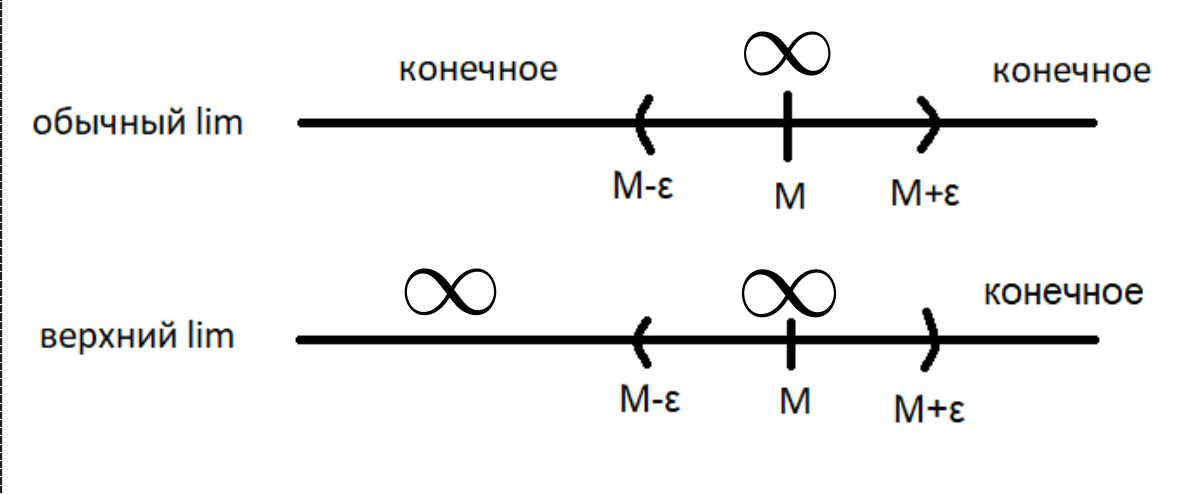
\includegraphics{2.9.1}\\
    Левее $M-\varepsilon$ в случае "обычного" предела находятся конечное число элементов $x_n$, а в случае верхнего предела - $\infty$ число элементов $x_n$.\\
    \textbf{Нижним пределом} последовательности $\{x_n\}$ называется число $m$ (конечное, $\pm \infty$):
    \begin{enumerate}
        \item $\exists$ подпоследовательность $\{x_{n_{k}}\} \Big| \lim_{k\to\infty}x_{n_{k}} = m$.
        \item $\forall$ сходящейся $\{x_{n_{k}}\} \lim_{k\to\infty} x_{n_{k}} \ge m$.\\
        Обозначение: $m = \underline{\lim}_{k\to\infty}x_n$.\\
        Замечание: если $\{x_n\}$ неограничена сверху, то $\underline{\lim}_{k\to\infty}x_n = -\infty$.\\
        Замечание: если $\{x_n\}$ сходящаяся и $\lim_{n\to\infty} x_n = m$, то $\underline{\lim}_{k\to\infty}x_n = m$.
    \end{enumerate}
    \subsubsection*{Разница между обычным пределом (единственным) и нижним пределом}
    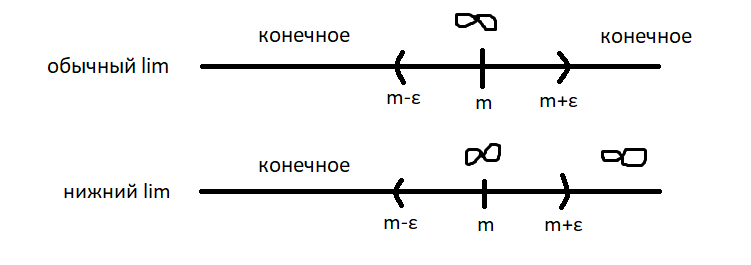
\includegraphics{2.9.2}\\
    Разница между "обычным" пределом и нижним пределом заключается в том, что правее $M+\varepsilon$ в случае "обычного" предела находятся конечное число элементов $x_n$, а в случае нижнего предела - $\infty$ число элементов $x_n$.\\
    Очевидно, $\underline{\lim}_{n\to\infty}x_n \le \overline{\lim}_{n\to\infty}x_n$.
    Для того, чтобы последовательность $\{x_n\}$ имела предел (конечный, $\pm \infty$) $\Leftrightarrow$ чтобы $\underline{\lim}_{n\to\infty} x_n = \overline{\lim}_{n\to\infty} x_n$. В этом случае $\lim_{n\to\infty} x_n = \underline{\lim_{n\to\infty}} x_n = \overline{\lim}_{n\to\infty} x_n$
    
    \subsection{Критерий Коши сходимости числовой последовательности}
    \noindent Последовательность $\{x_n\}$ называется \textbf{фундаментальной}, если она удовлетворяет условию Коши:
    \[ \forall \varepsilon > 0 \text{ } \exists \text{ } n_{0} \text{ } \big| \text{ } \forall n > n_{0}, \forall m > n_{0} \text{ } |x_n - x_{m}| < \varepsilon \]
    \begin{center}
        или
    \end{center}
    \[ \forall \varepsilon > 0 \text{ } \exists \text{ } n_{0} \text{ } \big| \text{ } \forall n > n_{0}, \forall p > 0 \text{ } |x_{n+p} - x_n| < \varepsilon \]
    \subsubsection*{Леммы о фундаментальных последовательностях}
    \noindent \textbf{Лемма 1:} если последовательность $\{x_n\}$ имеет конечный предел, то она фундаментальная.\par\noindent
    \underline{Доказательство:}
    \begin{adjustwidth}{1.5em}{1.5em}
        Пусть $\posl{x}{n}$ - сходящаяся.\\
        Тогда $\exists$ $\lim_{n\to\infty}x_n = a$, т.е.
        \[ \forall \varepsilon > 0 \text{ } \exists \text{ } N = N(\varepsilon) \text{ } \big| \text{ } \forall n > N \implies |x_{n} - a| < \frac{\varepsilon}{2} \]
        Пусть $m > N$ и $n > N$. Рассмотрим $|x_m - x_n|$.
        \[
            |x_m - x_n| = |(x_m - a) - (x_n - a)| \le |x_m - a| + |x_n - a| < \frac{\varepsilon}{2} + \frac{\varepsilon}{2} = \varepsilon
        \]
        Т.е. $\posl{x}{n}$ - фундаментальна.
        \begin{center}
            \textbf{Ч.т.д.}
        \end{center}
    \end{adjustwidth}

    \noindent \textbf{Лемма 2:} если последовательность фундаментальна, то она ограничена.\par\noindent
    \underline{Доказательство:}\par
    \begin{adjustwidth}{1.5em}{1.5em}
        Пусть $\posl{x}{n}$ - фундаментальна. Тогда по условию Коши
        \[ \exists \text{ } n_0 \text{ } \big| \text{ } \forall m,n > n_0 \implies |x_n - x_m| < \varepsilon \]
        Зафиксируем $m = n_0 + 1$. Получим $|x_n - x_{n_0+1}| < \varepsilon$.
        \begin{gather*}
            -\varepsilon < x_n - x_{n_0 + 1} < \varepsilon\\
            x_{n_0 + 1} - \varepsilon < x_n <  x_{n_0 + 1} + \varepsilon
        \end{gather*}
        Обозначим $d = max\{|x_1|, |x_2|, \dots, |x_{n_0}|, |x_{n_0+1} + \varepsilon|\}$.\\
        Тогда
        \[ \forall n \in N \Rightarrow -d \le x_n \le d \]
        То есть $\posl{x}{n}$ ограничена.
        \begin{center}
            \textbf{Ч.т.д.}
        \end{center}
    \end{adjustwidth}

    \noindent \textbf{Лемма 3:} если некоторая подпосл-ть фундаментальной посл-ти сходится, то предел этой подпосл-ти является пределом всей посл-ти.\par\noindent
    \underline{Доказательство:}
    \begin{adjustwidth}{1.5em}{1.5em}
        Пусть $\posl{x}{n}$ - фундаментальная последовательность. Пусть $\posl{x}{n_k}$ - её сходящаяся подпосл-ть.\\
        Пусть $\lim_{k\to\infty}x_{n_k} = a$\\
        Зададим $\varepsilon > 0$\\
        По условию Коши
        \[ \exists \text{ } n_0 \text{ } \big| \text{ } \forall m,n > n_0 \implies |x_n - x_m| < \frac{\varepsilon}{2} \]
        Т.к. $\lim_{k\to\infty}x_{n_k} = a$, т.е.
        \[ \exists \text{ } k_0 = k_0(\varepsilon) \implies |x_{n_k} - a| < \frac{\varepsilon}{2} \]
        Пусть $k_0$ будет таким, чтобы при $k > k_0 \implies n_k > n_0$\\
        \begin{gather*}
            |x_n - a| = |x_n - x_{n_k} + x_{n_k} - a| \le |x_n - x_{n_k}| + |x_{n_k} - a| < \frac{\varepsilon}{2} + \frac{\varepsilon}{2} = \varepsilon \implies \lim_{n\to\infty} x_n = a
        \end{gather*}
        \begin{center}
            \textbf{Ч.т.д.}
        \end{center}
    \end{adjustwidth}

    \subsubsection*{Теорема 10.1 (критерий Коши сходимости числовой посл-ти):}
    Для того, чтобы посл-ть имела конечный предел $\Leftrightarrow$ чтобы она была фундаментальна.\par\noindent
    \underline{Доказательство:}\par
    \begin{adjustwidth}{1.5em}{1.5em}
        \textbf{Докажем необходимость} ($\Rightarrow$).\\
        Пусть посл-ть имеет конечный предел. Тогда по лемме 1 она фундаментальна.\par\noindent
        \textbf{Докажем достаточность} ($\Leftarrow$).\\
        Пусть посл-ть фундаментальная. Тогда по лемме 2 она ограничена, следовательно по теореме Больцано-Вейерштрасса можно извлечь сходящуюся подпосл-ть.\\
        Тогда по лемме 3 вся посл-ть будет иметь предел, равный пределу подпосл-ти, т.е. посл-ть сходящаяся.
        \begin{center}
            \textbf{Ч.т.д.}
        \end{center}
    \end{adjustwidth}

    \section{Теория пределов функций. Непрерывность функций в точке и на отрезке.}
    \subsection{Функция. Предел функции в точке.}
    \noindent Пусть $E \subset R$. Пусть $\forall x \in E$ по вполне определённому закону ставится в соответствие единственное число $y$. Тогда говорят, что на множестве $E$ задана \textbf{функция} $y = f(x)$.\par\noindent
    $E$ - область определения функции.\\
    $x$ - независимая переменная (аргумент функции).\\
    $y$ - зависимая переменная (функция).
    \subsubsection*{Определение предела функции в точке по Гейне (в терминах последовательностей)}
    Число $a$ называется пределом функции $f(x)$ в точке $x_0$, если $f(x)$ определена в некоторой окрестности точки $x_0$, быть может за исключением самой точки $x_0$ (такая окрестность называется выколотой окрестностью) и $\forall \posl{x}{n} \text{ } \big| \text{ } \lim_{n\to\infty}x_n = x_0$, порождаемая ею посл-ть $\{f(x_n)\}$ имеет своим пределом точку $a$, т.е. $\lim_{n\to\infty}f(x_n) = a$.\\
    \underline{Запись:}
    \[ \lim_{x \to x_0}f(x) = a \]
    \begin{center}
        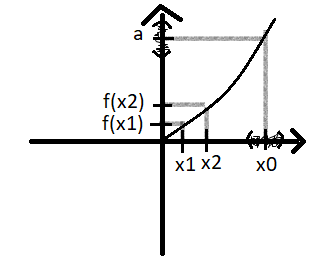
\includegraphics{3.1.1}
    \end{center}
    \underline{Пример:}
    \begin{adjustwidth}{1.5em}{1.5em}
        Рассмотрим такой предел
        \begin{gather*} 
            \lim_{x\to0}\frac{2x^2+x-1}{x-1} =
            \begin{vmatrix}
                \text{Пусть }x_n\text{ - произвольная}\\
                \lim_{n\to\infty}x_n = 0
            \end{vmatrix} =
            \lim_{n\to\infty} \frac{2x_n^2+x_n-1}{x_n-1} =\\
            \frac{\lim_{n\to\infty}(2x_n^2 + x_n - 1)}{\lim_{n\to\infty}(x_n-1)} = \frac{\lim_{n\to\infty}(2x^2_n)+\lim_{n\to\infty}x_n - 1}{\lim_{n\to\infty}x_n - 1} =\\
            \frac{2\lim_{n\to\infty}x_n \times \lim_{n\to\infty}x_n + \lim_{n\to\infty}x_n - 1}{\lim_{n\to\infty}x_n - 1} = \frac{-1}{-1} = 1
        \end{gather*}
        Другой пример: доказать, что $\lim_{x\to0}\sin\frac{1}{x} = \nexists$\par\noindent
        \underline{Доказательство:}
        \begin{adjustwidth}{1.5em}{1.5em}
            Выберем $\posl{x}{n}$ такую, что $\lim_{n\to\infty}x_n = 0$.\\
            \begin{enumerate}
                \item $x_n = \frac{1}{\pi n}$
                \[ \lim_{n\to\infty}\frac{1}{\pi n} \implies \lim_{n\to\infty}\sin \frac{1}{\frac{1}{\pi n}} = \lim_{n\to\infty}\sin \pi n = 0 \]
                \item $x_n = \frac{1}{\frac{\pi}{2} + 2\pi n}$
                \[ \lim_{n\to\infty}\frac{1}{\frac{\pi}{2} + 2\pi n} = 0 \implies \lim_{n\to\infty}\sin \frac{1}{\frac{1}{\frac{\pi}{2} + 2\pi n}} = \lim_{n\to\infty} \sin(\frac{\pi}{2} + 2\pi n) = \lim_{n\to\infty}\sin \frac{\pi}{2} = 1 \]
                Поэтому $\lim_{x\to 0}\sin \frac{1}{x} = \nexists$.
                \begin{center}
                    \textbf{Ч.т.д.}
                \end{center}
            \end{enumerate}
        \end{adjustwidth}
    \end{adjustwidth}
    
    \subsubsection*{Определение предела функции в точке по Коши}
    Число $a$ называется пределом функции $f(x)$ в точке $x_0$, если $f(x)$ определена в окрестности точки $x_0$, быть может за исключением самой точки $x_0$ и, если $\forall \varepsilon > 0$ $\exists$ $\delta = \delta(\varepsilon)$ $\big|$ $|x - x_0| < \delta \implies |f(x) - a| < \varepsilon$\\
    \begin{center}
        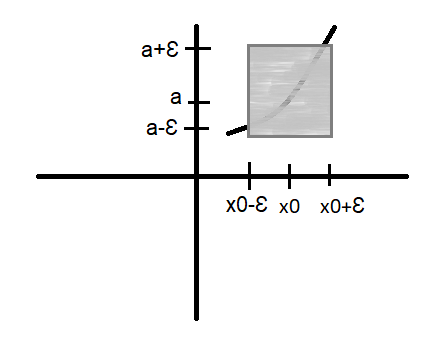
\includegraphics{3.1.2}
    \end{center}
    Если $x$ находятся в $\delta$-окрестности точки $x_0$, то все значения $f(x)$ располагаются в полосе шириной $2\varepsilon$.
    \subsubsection*{Теорема 1.1:}
    Определения предела функции $f(x)$ в точке $x_0$ по Гейне и по Коши эквивалентны.\par\noindent
    \underline{Доказательство:}
    \begin{adjustwidth}{1.5em}{1.5em}
        \begin{enumerate}
            \item \textbf{Докажем Гейне $\rightarrow$ Коши}\\
            Пусть функция имеет предел в точке $x_0$ в смысле Гейне.\\
            Предположим противное. Пусть функция $f(x)$ не имеет предел в точке $x_0$ в смысле Коши. Это значит, что $\exists$ хотя бы одно $\varepsilon_0$, для которого нельзя подобрать нужное $\delta$.\\
            То есть $\forall \delta$ среди $x$, удовлетворяющих неравенству $|x-x_0| < \delta$ должно найтись хотя бы одно $x = x(\delta) : |f(x(\delta)) - a| \ge \varepsilon$\\
            Составим последовательность. Выберем $\delta = \frac{1}{k}$ и для каждого $k$ будем искать точку $x_k$ для которой не выполняется определение Коши.
            \begin{enumerate}
                \item $k = 1$ $\delta = 1$ $|x_1 - x_0| < 1 \implies |f(x_1) - a| \ge \varepsilon_0$\\
                такой $x_1$ $\exists$
                \item $k = 2$ $\delta = \frac{1}{2}$ $|x_2 - x_0| < \frac{1}{2} \implies |f(x_2) - a| \ge \varepsilon_0$\\
                такой $x_2$ $\exists$
                \item $k = 3$ $\delta = \frac{1}{3}$ $|x_3 - x_0| < \frac{1}{3} \implies |f(x_3) - a| \ge \varepsilon_0$\\
                такой $x_3$ $\exists$
            \end{enumerate}
            То есть $\forall k > 0$ $|x_k - x_0| < \frac{1}{k} \implies \lim_{k\to\infty} x_k = x_0$, но тогда $|f(x_k) - a| \ge \varepsilon_0$, то есть $\lim_{k\to\infty} f(x_k) \ne a$. Получили противоречие, т.к. по Гейне $\lim_{k\to\infty} f(x_k) = a$.
            \item \textbf{Докажем Коши $\rightarrow$ Гейне}\\
            Пусть функция имеет предел по Коши.\\
            Зададим произвольную последовательность $\posl{x}{n} : \lim_{n\to\infty} x_n = x_0$.\\
            Так как определение по Коши выполняется, то
            \[
                \forall \varepsilon > 0 \text{ } \exists \text{ } \delta = \delta(\varepsilon) : |x - x_0| < \delta \implies |f(x) - a| < \varepsilon
            \]
            \begin{gather*}
                \text{Т.к. } \lim_{n\to\infty}x_n = x_0 \implies \forall \varepsilon > 0 \text{ } \exists n_0 = n_0(\varepsilon) : |x_n - x_0| < \delta \implies\\
                |f(x_n) - a| < \varepsilon \implies \lim_{x\to x_0} f(x) = a
            \end{gather*}
        \end{enumerate}
        \begin{center}
            \textbf{Ч.т.д.}
        \end{center}
    \end{adjustwidth}
    \subsubsection*{Предел функции в бесконечно удалённой точки}
    \[\lim_{x\to +\infty}f(x) = a\]
    Число $a$ называется пределом функции $f(x)$ при $x \to +\infty$, если 
    \[ \forall \varepsilon > 0 \text{ } \exists \text{ } k = k(\varepsilon) : x > k \implies |f(x) - a| < \varepsilon \]
    \underline{Упр.:} уметь расписывать \textbf{ВСЕГДА и ВЕЗДЕ}
    \begin{adjustwidth}{1.5em}{1.5em}
        \begin{gather*}
            \lim_{x\to -\infty}f(x) = a;
            \lim_{x\to x_0}f(x) = \infty;
            \lim_{x\to x_0}f(x) = -\infty;\\
            \lim_{x\to +\infty}f(x) = +\infty;
            \lim_{x\to +\infty}f(x) = -\infty;
            \lim_{x\to -\infty}f(x) = +\infty;\\
            \lim_{x\to -\infty}f(x) = -\infty
        \end{gather*}
        Например, распишем последнее.
        Нужны два параметра. В определении Коши есть $\delta$ для $x$ (аргумента) и $\varepsilon$ для $y$ (функции).\\
        Т.к. $x \to -\infty$, то мы не можем использовать $\delta$ (она используется для малых величин), поэтому введём параметр $K$ вместо $\delta$.\\
        Т.к. $\lim_{x\to -infty}f(x) = -\infty$, то мы не можем использовать $\varepsilon$ (он используется для малых величин), поэтому введём параметр $M$ вместо $\varepsilon$.\\
        Тогда определение принимает вид:
        \[
            \forall M > 0 \text{ } \exists \text{ } K = K(M) > 0 : x < -K \implies f(x) < -M
        \]
    \end{adjustwidth}

    \subsection{Односторонние пределы}
    Если значение функции $f(x)$ стремится к числу $a$ по мере стремления $x$ к $x_0$ со стороны меньших (больших) значений, то число $a$ называют пределом функции $f(x)$ в точке $x_0$ слева (справа)
    \begin{center}
        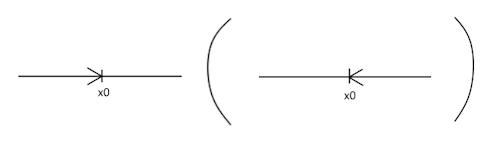
\includegraphics{3.2.1}
    \end{center}
    Обозначение:
    \begin{itemize}
        \item предел слева: $\lim_{x\to x_0 - 0}f(x) = f(x_0 - 0) = a$
        \item предел справа $\lim_{x\to x_0 + 0}f(x) = f(x_0 + 0) = a$
    \end{itemize}
    \underline{Пример:}
    \begin{adjustwidth}{1.5em}{1.5em}
        \[
            \lim_{x\to 0-0} 2^{\frac{1}{x}} = 0; \lim_{x\to 0+0} 2^{\frac{1}{x}} = \infty
        \]
        \begin{center}
            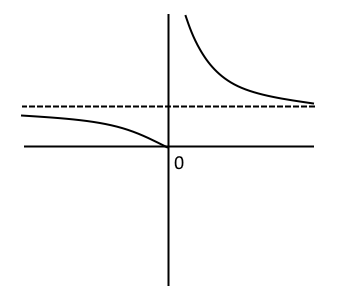
\includegraphics{3.2.2}
        \end{center}
    \end{adjustwidth}
    \underline{Пример 2:}
    \begin{adjustwidth}{1.5em}{1.5em}
        \[f(x) = \text{sign } x = \begin{cases}
            1, x > 0\\
            0, x = 0\\
            -1, x < 0
        \end{cases}
        \]
        \begin{center}
            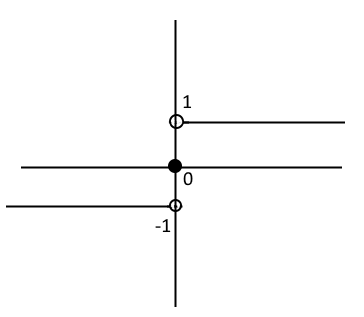
\includegraphics{3.2.3}
        \end{center}
        \[
            \lim_{x\to 0-0} \text{sign } x = -1; \lim_{x\to 0+0} \text{sign } x = 1
        \]
    \end{adjustwidth}
    \underline{Утверждение:} для того, чтобы существовал обычный двусторонний предел функции в точке $x_0$ $\Leftrightarrow$ чтобы в этой точке существовали левый и правый односторонние пределы и чтобы они были равны.
    \[ \lim_{x \to x_0} f(x) = a \Leftrightarrow \lim_{x \to x_0 - 0}f(x) = \lim_{x \to x_0 + 0} f(x) \]

    \subsection{Свойства пределов функций}
    \subsubsection*{Теорема 3.1}
    Если $\lim_{x\to x_0}f(x) = a$, где $a$ - конечное число, то в некоторой окрестности точки $x_0$ $f(x)$ ограничена.\par\noindent
    \underline{Доказательство:}
    \begin{adjustwidth}{1.5em}{1.5em}
        По определению Коши предела функции в точке:
        \[ \forall \varepsilon > 0 \text{ } \exists \text{ } \delta = \delta(\varepsilon) : |x - x_0| < \delta \implies |f(x) - a| < \varepsilon \]
        \[ -\varepsilon < f(x) - a < \varepsilon \]
        \[ a - \varepsilon < f(x) < a + \varepsilon \]
        \begin{center}
            \textbf{Ч.т.д.}
        \end{center}
    \end{adjustwidth}

    \subsubsection*{Теорема 3.2 (о сохранении знака)}
    Если функция $f(x)$ имеет в точке $x_0$ не равный нулю конечный предел $a$, то $\exists$ окрестность точки $x_0 : \forall x$, принадлежащего этой окрестности, выполняется
    \begin{gather*}
        f(x) > \frac{a}{2}, a > 0\\
        f(x) < \frac{a}{2}, a < 0
    \end{gather*}
    \underline{Доказательство:}
    \begin{adjustwidth}{1.5em}{1.5em}
        $\lim_{x\to x_0}f(x) = a$\\
        Обозначим $U(x_0)$ - окрестность точки $x_0$\\
        Тогда $\forall x \in U(x_0) : |f(x) - a| < \varepsilon = \frac{|a|}{2}$
        \[a - \frac{|a|}{2} < f(x) < a + \frac{|a|}{2}\]
        \begin{align*}
            a &> 0 & a &< 0\\
            f(x) &> a - \frac{a}{2} & f(x) &< a - \frac{a}{2}\\
            f(x) &> \frac{a}{2} & f(x) &< -\frac{|a|}{2}
        \end{align*}
        \begin{center}
            \textbf{Ч.т.д.}
        \end{center}
    \end{adjustwidth}

    \subsubsection*{Теорема 3.3}
    Если $f(x) = c$ (константа), то $\lim_{x\to x_0}f(x) = c$ - уже доказана.
    
    \subsubsection*{Теорема 3.4}
    Если $\lim_{x\to x_0}f(x) = a, \lim_{x \to x_0}g(x) = b$ и $\forall x \in R$ из окрестности точки $x_0$:
    \[ f(x) \le g(x) \implies a \le b \]

    \subsubsection*{Теорема 3.5}
    Если $\varphi (x) \le f(x) \le g(x)$ и $\lim_{x\to x_0}\varphi(x) = \lim_{x\to x_0} g(x) = a$, то $\lim_{x\to x_0}f(x) = a$.

    \subsubsection*{Теорема 3.6}
    Если существуют конечные пределы $\lim_{x\to x_0}f(x)$ и $\lim_{x\to x_0}g(x)$, то существуют конечные пределы
    \[\lim_{x\to x_0}(\lambda f(x) + \mu g(x)) = \lambda\lim_{x\to x_0}f(x) + \mu \lim_{x\to x_0}g(x)\]
    \[\lim_{x \to x_0}(f(x) * g(x)) = \lim_{x\to x_0} f(x) * \lim_{x\to x_0} g(x)\]
    \[\lim_{x\to x_0}\frac{f(x)}{g(x)} = \frac{\lim_{x\to x_0}f(x)}{\lim_{x\to x_0}g(x)}, \lim_{x\to x_0}g(x) \ne 0\]
    
    \noindent\textbf{Критерий Коши существования функции в точке}:
    \begin{adjustwidth}{1.5em}{1.5em}
        Для того, чтобы существовал конечный предел при $x \to x_0$ $f(x) \Leftrightarrow$ чтобы $f(x)$ была определена в окрестности точки $x_0$ за исключением быть может самой точки $x_0$ и 
        \[ \forall \varepsilon > 0 \text{ } \exists U_\delta(x_0): \forall x', x'' \in U_\delta(x_0) \implies x', x'' \ne x_0, |f(x') - f(x'')| < \varepsilon \]
    \end{adjustwidth}
    
    \subsection{Непрерывность функции в точке. Разрывы I и II родов.}
    \noindent Функция $f(x)$ называется непрерывной в точке $x_0$, если 
    \[\lim_{x\to\infty}f(x) = f(x_0)\]
    \[\lim_{x\to\infty}f(x) = f(\lim_{x\to\infty}x) = f(x_0)\]
    \noindent Т.е. для непрерывности в точке функции множества меняются знаками предела и функции
    \begin{enumerate}
        \item Через приращение\\
        $\varDelta x = x - x_0$ - приращение аргумента\\
        $\varDelta y = y - y_0$ - приращение функции\\
        Функция $f(x)$, направленная в точке $x_0$, если $\lim_{\delta x = 0} \delta y = 0$
        \item Определение Гейне\\
        Функция $f(x)$ называется непрерывной в точке $x_0$, если для $\forall$ последовательности $\lim_{x\to\infty} x_n = x_0$\\
        Порождающая её последовательность $f(x_n)$ $\lim_{n\to\infty} f(x_0) = f(x_0)$
        \item Определение Коши\\
        Функция $f(x)$ называется непрерывной в точке $x_0$ $\forall \varepsilon > 0$ $\exists$ $(\delta - \delta \varepsilon)$
    \end{enumerate}
    Функция $f(x)$ имеет в точке $x_0$ разрыв II рода, если хотя бы один из пределов (справа или слева) не существует или бесконечен.\par\noindent
    \underline{Пример 1:} рассмотрим при $x \ne 2$
    \begin{gather*}
        f(x) = \frac{x^2 - 4}{x-2}\\
        f(x) = \frac{x^2-4}{x-2} = x+2\\
        f(2) = \nexists\\
        \lim_{x\to 2-0} f(x) = \lim_{x\to 2-0}(x+2) = 4\\
        \lim_{x\to 2+0} f(x) = 4
    \end{gather*}
    \begin{center}
        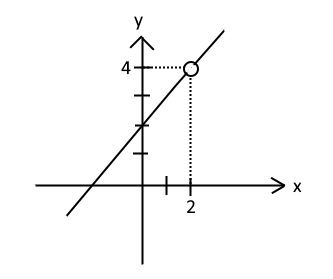
\includegraphics{3.4.2}
    \end{center}
    $f(x)$ непрерывна $\forall x \in R$, кроме $x=2$, где $f(x)$ терпит разрыв I рода устранений.\par\noindent
    \underline{Замечание:} рассмотрим 
    $ g(x) = \begin{cases}
        f(x), x \ne 2\\
        4, x = 2
    \end{cases}$;
    \noindent $g(x)$ непрерывна $\forall x \in R$\par\noindent
    \underline{Пример 2:} рассмотрим
    \[
        f(x) = [x] \text{ - целая часть }x, x > 0
    \]
    \begin{center}
        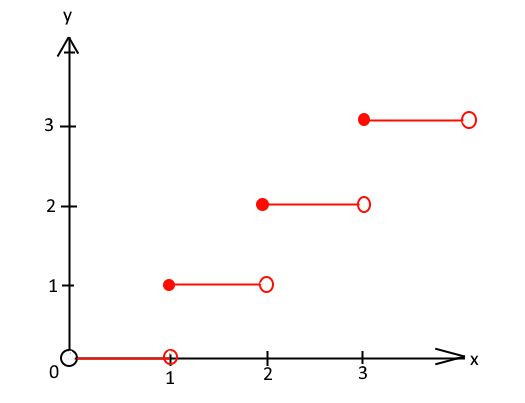
\includegraphics{3.4.3}
    \end{center}
    \begin{gather*}
        f(x) = 1\\
        \lim_{x\to 1-0} [x] = 0\\
        \lim_{x \to 1+0} [x] = 1
    \end{gather*}
    $\forall x \in N$ $f(x)$ терпит разрыв I рода (скачок), в остальных $x > 0$ $f(x)$ - непрерывна.\par\noindent
    \underline{Пример 3:} рассмотрим
    \[ f(x) = \frac{1}{x} \]
    \begin{center}
        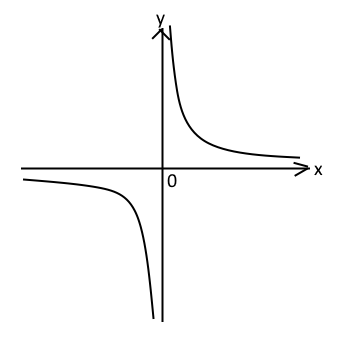
\includegraphics{3.4.4}
    \end{center}
    \begin{gather*}
        f(0) = \nexists\\
        \lim_{x \to 0-0} \frac{1}{x} = -\infty\\
        \lim_{x \to 0+0} \frac{1}{x} = \infty
    \end{gather*}
    $f(x)$ непрерывна $\forall x \in R$, кроме $x = 0$, где она терпит разрыв II рода.\\

    \subsection{Замечательные пределы}
    \subsubsection*{Теорема 5.1 (I Замечательный предел)}
    \[ \lim_{x\to 0}\frac{\sin x}{x} = \lim_{x\to 0} \frac{x}{\sin x} = 1 \]\noindent
    \underline{Доказательство:}
    \begin{adjustwidth}{1.5em}{1.5em}
        \begin{center}
            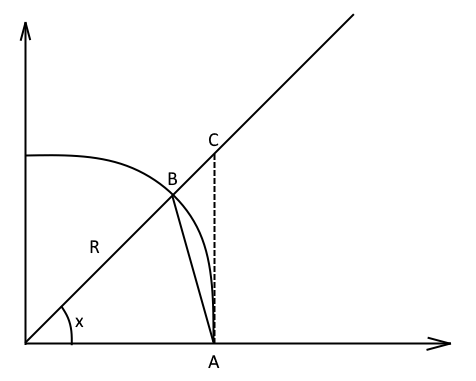
\includegraphics{3.5.1}
        \end{center}
        Рассмотрим в координатной плоскости круг радиуса $R$ с центром в начале координат\\
        \begin{gather*} 
            S_{\triangle OAB} < S_{\text{сект}OAB} < S_{\triangle OAC}\\
            \frac{1}{2}R^2\sin x < \frac{1}{2}R^2 x < \frac{1}{2} R^2 \text{tg } x\\
            \sin x < x < \text{tg } x \text{ } \big| : \sin x \text{ } (\text{пусть } \sin x > 0)\\
            1 < \frac{x}{\sin x} < \frac{1}{\cos x}\\
            \lim_{x\to 0} 1 = 1, \lim_{x\to 0} \frac{1}{\cos x} = 1 \implies \lim_{x\to 0} \frac{1}{\sin x} = 1
        \end{gather*}
        \begin{center}
            \underline{Замечание:} $f(x) = \cos x$ и $\frac{x}{\sin x}$, поэтому неравенство будет выполняться для $\frac{-\pi}{2} < x < 0$
        \end{center}
    \end{adjustwidth}

    \subsubsection*{Теорема 5.2 (II Замечательный предел)}
    \[ \lim_{x\to\infty}(1 + \frac{1}{x})^x = e \]
    \[ \lim_{x\to 0}(1 + x)^{\frac{1}{x}} = e \]\noindent
    \underline{Доказательство:}
    \begin{adjustwidth}{1.5em}{1.5em}
        Надо показать, что \[\lim_{x\to 0-0} (1 + x)^{\frac{1}{x}} = \lim_{x\to 0+0}(1+x)^{\frac{1}{x}} = e\]
        Замена: \[x = \frac{1}{y} \implies \lim_{y\to -\infty}(1 + \frac{1}{y})^y = \lim_{y\to\infty}(1 + \frac{1}{y})^y = e\]
        \underline{Замечание:} будем считать известным фактом, что $\forall n \in N$ верно $\lim_{n\to\infty}(1+\frac{1}{n})^n = e$.\par\noindent
        Пусть $x_n \to \infty$ (доказываем по определению Гейне)\\
        Покажем, что $\lim_{x_n\to\infty}(1 + \frac{1}{x_n})^{x_n} = e$. $\posl{x}{n}$ - произвольная посл-ть: $\lim_{n\to\infty}x_n = \infty$\\
        Рассмотрим посл-ть $k_n = [x_n]$ - целая часть $x_n$.\\
        \begin{gather*}
            k_n \le x_n < k_n + 1\\
            \frac{1}{k_n + 1} < \frac{1}{x_n} \le \frac{1}{k_n}\\
            1 + \frac{1}{k_n + 1} < 1 + \frac{1}{x_n} \le 1 + \frac{1}{k_n}\\
            (1 + \frac{1}{k_n + 1})^{k_n} < (1 + \frac{1}{x_n})^{k_n} \le (1 + \frac{1}{k_n})^{k_n}\\
            \text{т.к. } k_n \le x_n < k_n + 1\\
            (1 + \frac{1}{k_n + 1})^{k_n} < (1 + \frac{1}{x_n})^{k_n} \le (1 + \frac{1}{k_n})^{k_n+1}\\
        \end{gather*}
        \begin{enumerate}
            \item \[\lim_{n\to\infty}(1+\frac{1}{k_n+1})^{k_n+1-1} = \lim_{n\to\infty}(1+\frac{1}{k_n+1})^{k_n+1}(1+\frac{1}{k_n+1})^{-1} = e \times 1 = e\]
            \item \[\lim_{n\to\infty}(1+\frac{1}{k_n})^{k_n+1} = \lim_{n\to\infty}(1+\frac{1}{k_n})^{k_n}(1+\frac{1}{k_n})^{1} = e \times 1 = e\]
        \end{enumerate}
        Тогда $\lim_{x_n \to \infty}(1 + \frac{1}{x_n})^{x_n} = e$ (по теореме о двух милиционерах)
        Рассмотрим $x_n \to -\infty$. Замена: $x_n' = -x_n$.\\
        Рассмотрим $\lim_{x_n \to -\infty}(1+\frac{1}{x_n})^{x_n} = \lim_{x_n'\to\infty}(1 + \frac{1}{-x_n'})^{-x_n'} = e$\\
        \begin{center}
            \textbf{Ч.т.д.}
        \end{center}
    \end{adjustwidth}

    \subsection{Эквивалентные бесконечно малые функции в точке}
    \noindent Функция $f(x)$ называется беск. малой при $x \to x_0$, если $\lim_{x \to x_0}f(x) = 0$\\
    \underline{Замечание:} Функция, которая является беск. м. в одной точке, может не быть беск. б. в другой точке.\par\noindent
    \subsubsection*{Теорема 6.1}
    Сумма и произведения конечного числа беск. м. функция в точке есть функция беск. м. в точке.
    \subsubsection*{Теорема 6.2}
    Произведение беск. м. функции в точке на ограниченную есть беск. м. функция в точке.\par\noindent
    \underline{Доказательство:}
    \begin{adjustwidth}{1.5em}{1.5em}
        Пусть $f(x)$ - беск. м. функция в точке $x_0 \implies \lim_{x\to x_0}f(x)=0$\\
        Пусть $g(x)$ - ограничена в окрестности точки $x_0$ ($u(x_0)$) $\implies \exists$ $M : |g(x)| \le M$\\
        $0 \le |f(x)g(x)| \le M|f(x)|$\\
        По теореме о двух милиционерах так как $\lim_{x\to x_0}0 = 0$ и $\lim_{x\to x_0}M|f(x)| = M \times 0 = 0$, то $\lim_{x\to x_0}|f(x)g(x)| = 0 \implies \lim_{x\to x_0}f(x)g(x) = 0$
        \begin{center}
            \textbf{Ч.т.д.}
        \end{center}
    \end{adjustwidth}
    \underline{Пример:}
    \begin{adjustwidth}{1.5em}{1.5em}
        \[\lim_{x\to0} x\sin \frac{1}{x} = 0\]
        $x$ - беск. м.\\
        $\sin \frac{1}{x}$ - огр.
    \end{adjustwidth}
    \subsubsection*{Эквивалентность беск. м. функций}
    \noindent Пусть $f(x)$ и $g(x)$ являются беск. м. функциями в точке $x_0$. Тогда они называются эквивалентными беск. м. функциями в точке $x_0$, если
    \[ \lim_{x\to x_0}\frac{f(x)}{g(x)} = 1 \]
    Обозначение: $f(x) \sim g(x), x \to x_0$\\
    Например, $\sin x \sim x, x \to 0$
    \begin{center}
        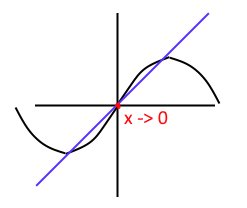
\includegraphics{3.6.1}
    \end{center}
    \underline{Замечание:} если $f_1(x) \sim f_2(x), x \to x_0$, а $g_1(x) \sim g_2(x), x \to x_0$, то
    \[ \lim_{x\to x_0}\frac{f_1(x)}{g_1(x)} = \lim_{x\to x_0}\frac{f_2(x)}{g_2(x)} = \lim_{x\to x_0}\frac{f_2(x)}{g_1(x)} = \lim_{x\to x_0}\frac{f_1(x)}{g_2(x)} \]
    \begin{adjustwidth}{1.5em}{1.5em}
        При нахождении предела дроби можно заменять на эквивалентные беск. м. или числитель, или знаменатель, или и то, и другое (но не часть числителя или знаменателя).
        \begin{center}
            Так \textbf{НЕЛЬЗЯ}:
        \end{center}
        \[ \text{tg } x - \sin x \sim^? 0 \]
    \end{adjustwidth}
    Основные эквивалентности при $x \to 0$
    \begin{enumerate}
        \item $\sin x \sim x$
        \item $\tg x \sim x$
        \item $\ln(1+x) \sim x$
        \item $e^x - 1 \sim x$
        \item $a^x - 1 \sim x \ln a$
        \item $(1+x)^m - 1 \sim mx$
        \item $\arcsin x \sim x$
        \item $\arctan x \sim x$
        \item $1 - \cos x \sim \frac{x^2}{2}$
    \end{enumerate}
    \underline{Доказательство:}
    \begin{adjustwidth}{1.5em}{1.5em}
        \begin{enumerate}
            \item доказано (I Замечательный предел)
            \item \[\lim_{x\to 0}\frac{\text{tg } x}{x} = \lim_{x\to 0}\frac{\sin x}{x \cos x} = 1\]
            \item \[\lim_{x\to 0}\frac{\ln(1+x)}{x} = \lim_{x\to 0}\frac{1}{x} \times \ln(1+x) = \lim_{x\to 0}\ln(1+x)^{\frac{1}{x}} = \ln \lim_{x\to 0}(1+x)^{\frac{1}{x}} = \ln e = 1\]
            \item частный случай пункта 5 $(a = e)$
            \item \[\lim_{x\to 0}\frac{a^x-1}{x \ln a} = \begin{vmatrix}
                a^x - 1 = y\\
                x \to 0 \implies y \to 0\\
                \ln a^x = \ln(1+y)\\
                x\ln a = \ln(1+y)
            \end{vmatrix} = \lim_{y\to 0}\frac{y}{\ln(1+y)} = 1\]
            \item \begin{gather*}
                \lim_{x\to 0}\frac{(1+x)^m-1}{mx} = \lim_{x\to 0}\frac{(1+x)^m-1}{\ln(1+x)}\frac{\ln(1+x)}{mx} =\\= \lim_{x\to 0}\frac{(1+x)^m-1}{\ln (1+x)} \lim_{x\to 0}\frac{\ln(1+x)}{mx} = \lim_{x\to 0}\frac{(1+x)^m-1}{m\ln(1+x)} = \begin{vmatrix}
                    (1+x)^m - 1 = y\\
                    x \to 0 \implies y \to 0\\
                    (1+x)^m = y + 1\\
                    \ln(1+x)^m = \ln(1+y)\\
                    m\ln(1+x) = \ln(1+y)
                \end{vmatrix} =\\= \lim_{y\to 0}\frac{y}{\ln(1+y)} = 1
            \end{gather*}
            \item \[\lim_{x\to 0}\frac{\arcsin x}{x} = \begin{vmatrix}
                \arcsin x = y\\
                x \to 0 \implies y \to 0\\
                x = \sin y
            \end{vmatrix} = \lim_{y\to 0}\frac{y}{\sin y} = 1\]
            \item \[\lim_{x\to 0}\frac{\arctan x}{x} = \begin{vmatrix}
                \arctan x = y\\
                x \to 0 \implies y \to 0\\
                x = \text{tg } y
            \end{vmatrix} = \lim_{y\to 0}\frac{y}{\text{tg } y} = \lim_{y\to 0}\frac{y\cos y}{\sin y} = 1\]
            \item \[\lim_{x\to 0}\frac{1-cos x}{\frac{x^2}{2}} = \lim_{x\to 0}\frac{2\sin^2(\frac{x}{2})}{\frac{x^2}{2}} = 1\]
        \end{enumerate}
    \end{adjustwidth}

    \subsection{Порядок переменной. Сравнение функций в окрестности заданной точки.}
    \noindent Рассмотрим функции $f(x)$ и $g(x)$, заданные в $u(x_0)$ за исключением быть может самой точки $x_0$.\par\noindent
    $x_0$ - конечная, $\pm \infty$.\\
    Пусть $g(x) \ne 0$ $\forall x \in u(x_0)$.\par\noindent
    Если $\lim_{x\to x_0}\frac{f(x)}{g(x)} = \left[ \frac{0}{0} \right] = 0$, то в этом случае $f(x) = o(g(x))$, ($o$ читается как "$o$ малое"), т.е. $f(x)$ является беск. м. более высокого порядка малости, чем $g(x)$ при $x \to x_0$.\par\noindent
    Если $\lim_{x\to x_0}\frac{f(x)}{g(x)} = k \ne 0$, то $f(x)$ и $g(x)$ называются беск. малой одного порядка при $x \to x_0$.\par\noindent
    Беск. малая $f(x)$ при $x \to x_0$ имеет $k$-ый порядок малости по отношению к $g(x)$ при $x \to x_0$, если $f(x)$ имеет тот же порядок малости, что и $g^k(x)$, т.е. $\lim_{x\to x_0}\frac{f(x)}{g^k(x)} = 0$
    
    \subsubsection*{Теорема 7.1}
    Для того, чтобы функции $f(x)$ и $g(x)$ были эквивалентными при $x \to x_0 \Leftrightarrow f(x) = g(x) + o(g(x)), x \to x_0$\par\noindent
    \underline{Доказательство:}
    \begin{adjustwidth}{1.5em}{1.5em}
        \textbf{Докажем необходимость ($\Rightarrow$)}\par\noindent
        Пусть $f(x) \sim g(x), x \to x_0$. Тогда по определению $\lim_{x \to x_0}\frac{f(x)}{g(x)} = 1$.\\
        Следовательно, \begin{gather*}
            \lim_{x\to x_0}\varepsilon(x) = 0\\
            \frac{f(x)}{g(x)} = 1 + \varepsilon(x) \Big| \times g(x)\\
            f(x) = g(x) + \varepsilon(x) g(x) = g(x) + o(g(x))
        \end{gather*}\noindent
        \textbf{Докажем достаточность ($\Leftarrow$)}\par\noindent
        Пусть $f(x) = g(x) + o(g(x)), x \to x_0$\\
        Например, 
        \begin{gather*}
            f(x) = g(x) + \varepsilon(x) g(x) \Big| : g(x)\\
            \frac{f(x)}{g(x)} = 1 + \varepsilon(x)\\
            \lim_{x \to x_0} \frac{f(x)}{g(x)} = 1
        \end{gather*}
        Т.е. $f(x) \sim g(x), x \to x_0$.
        \begin{center}
            \textbf{Ч.т.д.}
        \end{center}
    \end{adjustwidth}

    Функция $f(x)$ называется функцией, ограниченной относительно функции $g(x)$ в $u(x_0)$, если ограничена функция $\frac{f(x)}{g(x)}$, т.е.
    \[ \left|\frac{f(x)}{g(x)}\right| \le c \text{ или } \left|f(x)\right| \le c\left|g(x)\right| \]
    В этом случае $f(x) = O(g(x)), x \to x_0$\\
    $f(x) = O(1), x \to x_0$ = "функция $f(x)$ ограничена.

    \subsection{Глобальные свойства функций, непрерывных на отрезке}
    \noindent Функция $f(x)$ называется непрерывной на отрезке $[a; b]$, если она непрерывна в каждой точке интервала $(a; b)$, в точке $x = a$ справа, в точке $x = b$ слева.
    \subsubsection*{Теорема 8.1 (I-ая теорема Вейерштрасса)}
    Если функция $f(x)$ непрерывна на $[a; b]$, то она ограничена на нём, т.е.
    \[ \exists M > 0 : \left|f(x)\right| \le M \text{ } \forall x \in [a; b] \]\noindent
    \underline{Доказательство:}
    \begin{adjustwidth}{1.5em}{1.5em}
        Предположим противное. Пусть $f(x)$ непрерывна на $[a; b]$, но при этом не ограничена на нём.\\
        Составим последовательность $x_n$ следующим образом:
            \begin{gather*}
                \exists x_1 \in [a; b] : f(x_1) > 1\\
                \exists x_2 \in [a; b] : f(x_2) > 2\\
                \vdots\\
                \exists x_n \in [a; b] : f(x_n) > 2\\
                \vdots
            \end{gather*}
        В результате получили посл-ть $\posl{x}{n}$. Она ограничена ($\forall n$ $x_n \in [a; b]$). По теореме Больцано-Вейерштрасса (т. 8.1 гл. 2) из неё можно извлечь сходяющуся подпосл-ть $x_{n_k}$\\
        Пусть $\lim_{k\to\infty}x_{n_k} = \alpha$\\
        Так как $f(x)$ непрерывна на $[a; b]$, то по определению $\lim_{x\to x_0} f(x) = f(x_0)$\\
        В нашем случае $\lim_{k\to\infty} f(x_{n_k}) = f(\lim_{k\to\infty}x_{n_{k}}) = f(\alpha)$ - конечное число (в силу непрерывности)\\
        Однако $f(\alpha)$ является беск. б. по построению $x_n$ ($f(x_n)$ беск. б.), $f(\alpha) = \infty$.\\
        Получили противоречие, т.е. $f(x)$ ограничена.
        \begin{center}
            \textbf{Ч.т.д.}
        \end{center} 
    \end{adjustwidth}
    \subsubsection*{Теорема 8.2 (II-ая теорема Вейерштрасса)}
    Среди значений, которые на отрезке $[a; b]$ принимает непрерывная функция, существует наибольшее и наименьшее значения (в том числе может быть и в крайних точках).\par\noindent
    \underline{Доказательство:}
    \begin{adjustwidth}{1.5em}{1.5em}
        По I-ой теореме Вейерштрасса $f(x)$ ограничена сверху, т.е. $\exists k : f(x) \le k \text{ }  \forall x \in [a; b]$\\
        Тогда существует точная верхняя грань $f(x)$ на $[a; b]$. $M = \sup f(x), x \in [a; b]$\\
        Составим вспомогательную посл-ть $\posl{x}{n}$ на основе свойства $\sup f(x)$.
        \begin{gather*}
            \exists x_1 : M - 1 < f(x_1) \le M\\
            \exists x_2 : M - \frac{1}{2} < f(x_2) \le M\\
            \vdots\\
            \exists x_n : M - \frac{1}{n} < f(x_n) \le M\\
            \vdots
        \end{gather*}
        $\posl{x}{n}$ ограничена ($\forall n x_n \in [a; b]$)\\
        Тогда по теореме Больцано-Вейерштрасса из неё можно извлечь сходящуюся подпосл-ть $x_{n_k}, \lim_{k\to\infty}x_{n_k} = \alpha$
        \begin{enumerate}
            \item С одной стороны, $f(x)$ непрерывна на $[a; b] \implies \lim_{k\to\infty}f(x_{n_k}) = f(\lim_{k\to\infty}x_{n_k}) = f(\alpha)$
            \item С другой стороны $M - \frac{1}{n} < f(x_n) \le M$, следовательно
            \[
                M - \frac{1}{n_k} < f(x_{n_k}) \le M
            \]
            Т.к. $\lim_{k\to\infty} (M - \frac{1}{n_k}) = M$ и $\lim_{k\to\infty} M = M$, то $\lim_{k\to\infty}f(x_{n_k}) = M$ (по т. о двух милиционерах), т.е. $f(\alpha) = M$.\\
            $\beta \in [a; b] : f(\beta) = m$
        \end{enumerate}
    \end{adjustwidth}
    \subsubsection*{Теорема 8.3 (Теорема Больцано-Коши)}
    Если функция $f(x)$ непрерывна на $[a; b]$ и $f(a) = m, f(b) = n$, то на интервале $(a; b)$ $f(x)$ по крайней мере один раз принимает значение $p$, заключённое между $m$ и $n$.
    \begin{center}
        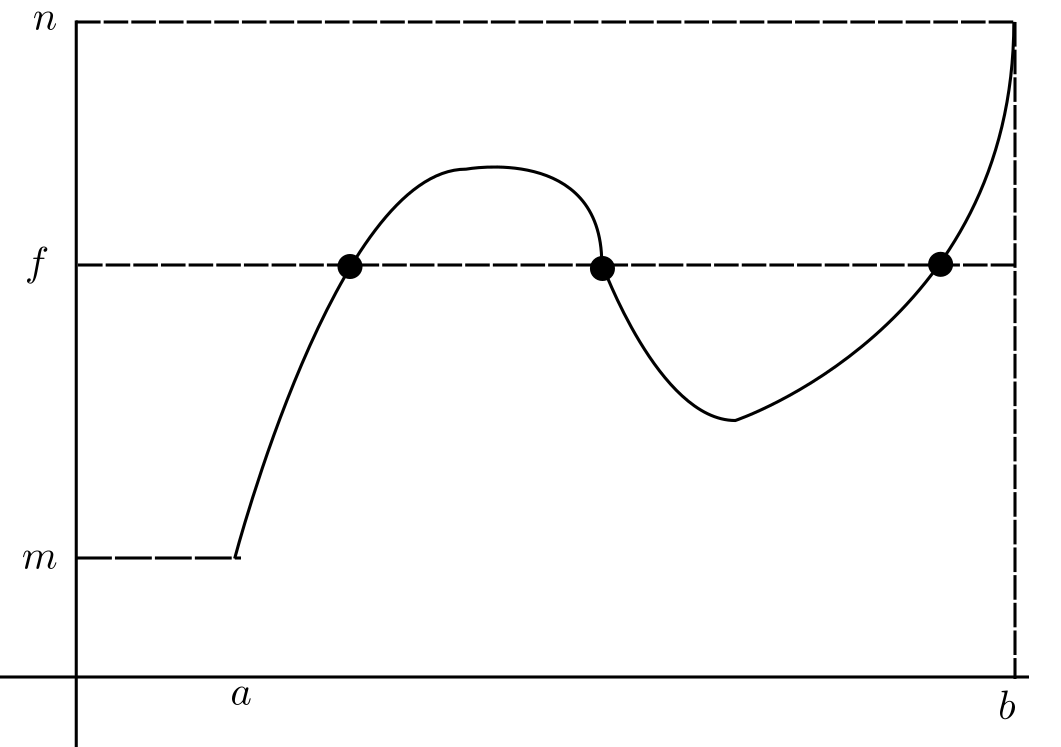
\includegraphics{3.8.1}
    \end{center}
    \underline{Доказательство:}
    \begin{adjustwidth}{1.5em}{1.5em}
        Для доказательства надо найти точку $\xi$, $f(\xi) = p$.\\
        Разобъём отрезок $[a; b]$ на 2 равных отрезка точкой $\frac{a + b}{2}$\\
        Варианты:
        \begin{enumerate}
            \item $f(\frac{a+b}{2}) = p \implies \xi = \frac{a+b}{2}$. \textbf{Ч.т.д.}
            \item $f(\frac{a+b}{2}) \ne p$. Тогда либо $f(\frac{a+b}{2}) < p$, либо $f(\frac{a+b}{2}) > p$.\\
            В первом случае далее выберем отрезок $[\frac{a+b}{2}; b]$, во втором - $[a; \frac{a+b}{2}]$. Переобозначим выбранный отрезок $[a_1; b_1]$, $f(a_1) < p < f(b_1)$. $b_1 - a_1 = \frac{b-a}{2}$.\\
            Разделим $[a_1; b_1]$ на 2 равных отрезка и выберем тот, на левом конце которого значение функции меньше $p$, а на правом - больше.\\
            Тогда либо через конечное число шагов мы получим такую точку $\xi$, либо систему вложенных отрезков $[a_n; b_n], f(a_n) < p < f(b_n), b_n - a_n = \frac{b-a}{2^n} \to_{n \to \infty} 0$\\
            Тогда по теореме о вложенных отрезках $\exists$ точка $\xi$, принадлежащая всем отрезкам одновременно и $\lim_{n\to\infty}a_n = \lim_{n\to\infty} b_n = \xi$\\
            В точке $\xi$ $f(x)$ непрерывна.
            \[ \lim_{n\to\infty}a_n = \lim_{n\to\infty}b_n = f(\xi) \]
            Тогда по теореме о двух милиционерах:
            \[ f(a_n) < p < f(b_n) \implies \lim_{n\to\infty}p = f(\xi) \]
        \end{enumerate}
        \begin{center}
            \textbf{Ч.т.д.}
        \end{center}
    \end{adjustwidth}
    \textbf{Следствие теоремы Больцано-Коши:} если функция непрерывна на отрезке и на его концах принимает значения разных знаков, то на этом отрезке существует хотя бы одна точка такая, что значение $f(x)$ в этой точке равно 0.\par\noindent
    \underline{Замечание:} будем считать элементарные функции непрерывными на своей области определения: $\lim_{x\to x_0}\text{tg }\dots = \text{tg } \lim_{x\to x_0}\dots$\\
    \underline{Замечание:} замена неопределённостей может идти по такому принципу
    \begin{gather*}
        u^v \to e^{\ln u * v}\\
        1^\infty \to \left[0 \times \infty\right] \to \begin{cases}
            \left[\frac{0}{0}\right]\\
            \left[\frac{\infty}{\infty}\right]
        \end{cases}\\
        \infty^0 \to \left[\infty \times 0\right]\\
        0^0 \to \left[\infty \times 0\right]
    \end{gather*}

    \subsection{Равномерная непрерывная функция}\noindent
    Вспомним определение непрерывности функции в точке по Коши:
    \[ \forall \varepsilon > 0 \text{ } \exists \text{ } \delta = \delta(\varepsilon) : |x - x_0| < \delta \implies |f(x) - f(x_0)| < \varepsilon \]
    Зафиксируем $\varepsilon$. Вообще говоря, в каждой точке $x$ существует своё $\delta$, т.е. $\delta = \delta(\varepsilon, x)$.\\
    В связи с этим выделяют класс функций (непрерывных), для которых при фиксированном $\varepsilon > 0$ можно указать $\delta > 0$, пригодная сразу для всех $x$, принадлежащая некоторому $X$.\par\noindent
    Функция, определённая на множестве $X$, называется \textbf{равномерно-непрерывной} на этом множестве, если
    \[ \forall \varepsilon > 0 \text{ } \exists \text{ } \delta = \delta(\varepsilon) : \forall x', x'' \in X : |x' - x''| < \delta \implies |f(x') - f(x'')| < \varepsilon \]
    \begin{center}
        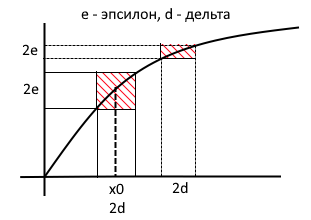
\includegraphics{3.9.1.png}
    \end{center}
    \underline{Примеры:}
    \begin{enumerate}
        \item $f(x) = x, x \in R$\\
        Пусть $x', x'' \in R : |x' - x''| < \delta$
        \[
            |f(x') - f(x'')| = |x' - x''| < \delta = \varepsilon
        \]
        \begin{center}
            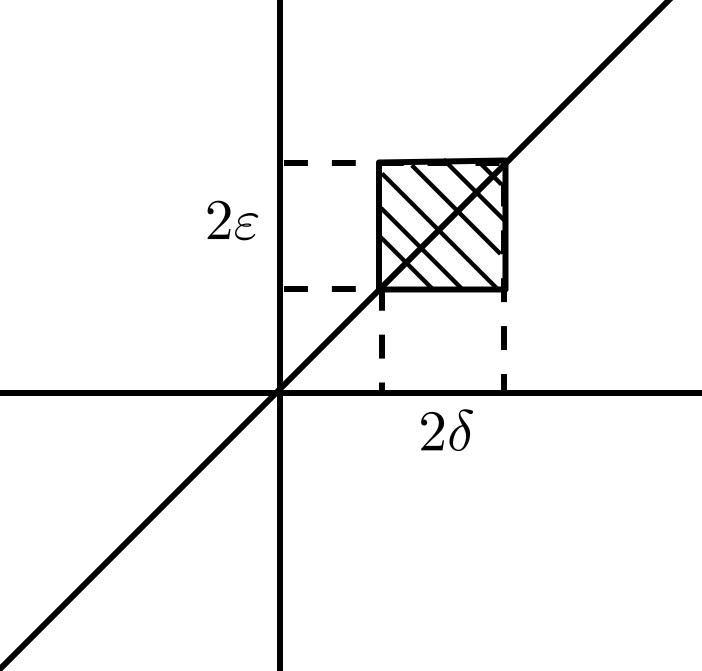
\includegraphics{3.9.2.png}
        \end{center}
        \item $f(x) = x^2, x \in R$\\
        Пусть $x', x'' \in R : |x' - x''| < \delta$\\
        Пусть $x'' = x' + h \implies |x' - x' - h| = |h| < \delta$
        \[ |f(x') - f(x'')| = |x'^2 - (x' + h)^2| = |x'^2 - x'^2 - 2x'h - h^2| = |2x'h + h^2| \]
        Так как $x' \in R$, то можно так его выбрать, что $|2x'h + h^2| = \infty \implies$ функция $f(x) = x^2$ не является непрерывной на области своего определения.
    \end{enumerate}
    \subsubsection*{Теорема 9.1 (Теорема Кантера)}
    Если функция определена и непрерывна на отрезке $[a; b]$, то она равномерно-непрерывна на нём.\par\noindent
    \underline{Доказательство:}
    \begin{adjustwidth}{1.5em}{1.5em}
        Предположим противное. Пусть \[\forall \varepsilon > 0 \text{ } \exists \text{ } \delta = \delta(\varepsilon) : \forall x', x'' \in [a;b] :  |x' - x''| < \delta \implies |f(x') - f(x'')| \ge \varepsilon \]
        Зададим последовательность $\delta_n : \lim_{n\to\infty} \delta_n = 0$.\\
        Построим две вспомогательные последовательности $x_n'$ и $x_n''$:
        \[ \exists \text{ } x_1', x_1'' : |x_1' - x_1''| < \delta_1 \implies |f(x_1') - f(x_1'')| \ge \varepsilon \]
        \[ \exists \text{ } x_2', x_2'' : |x_2' - x_2''| < \delta_2 \implies |f(x_2') - f(x_2'')| \ge \varepsilon \]
        \[ \exists \text{ } x_n', x_n'' : |x_n' - x_n''| < \delta_n \implies |f(x_n') - f(x_n'')| \ge \varepsilon \]
        Рассмотрим $\posl{x'}{n}$: она ограничена. Тогда по теореме. Больцано-Вейерштрасса из неё можно извлечь сх-ся подпосл-ть $\posl{x'}{n_k}$.\\
        Пусть $\lim_{k\to\infty} x'_{n_k} = x_0$\\
        Аналогично м. извлечь $\posl{x''}{n_k}$\\
        Т.к. $|x_n' - x_n''| < \delta_n \implies |x_{n_k}' - x_{n_k}''| < \delta_{n_k}$\\
        $\lim_{k\to\infty}x_{n_k}' = \lim_{k\to\infty}x_{n_k}'' = x_0$\\
        Так как $f(x)$ непрерывнв на $[a; b]$, то она непрерывна в точке $x_0 \in [a;b]$\\
        Значит $\lim_{k\to\infty}f(x'_{n_k}) = \lim_{k\to\infty}f(x''_{n_k}) = f(x_0)$\\
        Рассмотрим $|f(x') - f(x'')| \ge \varepsilon$ (*)
        \begin{adjustwidth}{1.5em}{1.5em}
            Перейдем в (*) к пределу при $k \to \infty$
            \[ \varepsilon \le | \lim_{k\to\infty}f(x'_{n_k}) - \lim_{k\to\infty}f(x''_{n_k})| = |f(x_0) - f(x_0)| = 0 \]
            Получили противоречие, т.к. $\varepsilon > 0 \implies f(x)$ - непрерывна.
        \end{adjustwidth}
    \end{adjustwidth}
    \underline{Пример:} рассмотрим $g = \sin \frac{1}{x}, x \in (0; 1)$
    \begin{adjustwidth}{1.5em}{1.5em}
        На $(0; 1)$ $y$ является непрерывна. Покажем, что на $(0; 1)$ $y$ не является равномерно-непрерывной функцией.\\
        Рассмотрим $x'_n$:
        \[x'_n = \frac{1}{\pi n}, \lim_{n\to\infty} x'_n = 0, x_n' \in (0; 1)\]
        Рассмотрим $x''_n$: 
        \[x''_n = \frac{1}{\frac{\pi}{2}+2\pi n}, \lim_{n\to\infty}x_n'' = 0, x''_n \in (0; 1)\]
        Рассмотрим 
        \[|f(x_n') - f(x_n'')| = |\sin \pi n - \sin (\frac{\pi}{2} + 2\pi n)| = 1\]
        \[ \forall \delta : |x_n' - x_n''| < \delta \implies |f(x'_n) - f(x''_n)| = 1 \]
        \[ \forall \varepsilon : 0 < \varepsilon < 1 \implies \nexists \delta(\varepsilon) \]
        Пусть $\varepsilon = \frac{1}{2}$. Тогда $\delta(\varepsilon) = \nexists$.
        \begin{center}
            \textbf{Ч.т.д.}
        \end{center}
    \end{adjustwidth}
    \underline{Замечание:} на практике, как правило, функции, которые растут больше, чем $y=x$, не является равн.-непр-ми на $D(f)$.

    \section{Дифференциальные исчисления функции}
    \subsection{Производная функции в точке}
    \noindent $y = f(x)$\\
    $\Delta x$ - приращение аргумента\\
    $\Delta y = f(x_0 + \Delta x) - f(x_0)$ - приращение функции\par\noindent
    \textbf{Производной} от функции $f(x)$ в точке $x_0$ называется предел отношения приращения функции в точке $x_0$ к приращению аргумента при стремлении последнего к 0.
    \[ \lim_{\Delta x \to 0} \frac{\Delta y}{\Delta x} = \lim_{\Delta x \to 0} \frac{f(x_0 + \Delta x) - f(x_0)}{\Delta x} = y' = \frac{dy}{dx} = \frac{d\sqcup}{dx}f \]
    \[ y'''' = y^{IV} = y^{(4)}  \]
    \underline{Замечание:} для существования производной от $f(x)$ в точке $x_0$ необходимо, чтобы $f(x)$ была определена в некоторой окрестности $x_0$ и в самой точке $x_0$.\\
    \underline{Замечание:} функция имеет производную в точке $x_0$, если $\exists$ $\lim_{\Delta x \to 0} \frac{\Delta y}{\Delta x}$\\
    \underline{Замечание:} если $\lim_{\Delta x \to 0}\frac{\Delta y}{\Delta x} = \pm \infty$, то говорят, что функция имеет бесконечную производную в точке.\par\noindent
    Если $\Delta x \to 0$ принимает только положительные значения то соответствующий предел называется правой производной от $f(x)$ в точке $x_0$.\\
    Если $\Delta x \to 0$ принимает только отрицательные значения то соответствующий предел называется левой производной от $f(x)$ в точке $x_0$.\par\noindent
    Функция $f(x)$ имеет производную на $[a; b]$, если она имеет производную во всех точках $(a; b)$, в точке $x=a$ имеет правую производную, в точку $x=b$ - левую.\par\noindent
    \underline{Утверждение:} если $f(x)$ имеет в точке $x_0$ правую и левую производные, то $f(x)$ имеет в точке $x_0$ производную.\\
    \underline{Утверждение:} если правая и левая производные в точке $x_0$ $\exists$ и не равны между собой, то производная в точке $x_0$ $\exists$.\\
    \underline{Пример:}
    \begin{adjustwidth}{1.5em}{1.5em}
        \begin{center}
            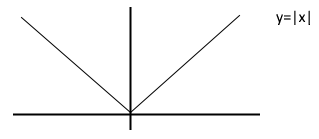
\includegraphics{4.1.1.png}
        \end{center}
        \[ \begin{matrix}
            y'\\
            \\
        \end{matrix}\Big|\begin{matrix}
            \\
            x = 0
        \end{matrix} \]
        Правая производная
        \[ \begin{matrix}
            y'_+\\
            \\
        \end{matrix}\Big|\begin{matrix}
            \\
            x = 0
        \end{matrix} = \lim_{\Delta x \to 0}\frac{f(x_0) - f(0)}{x_0 - 0} = \begin{vmatrix}
            \Delta x \to 0 \sim x_0 \to 0\\
            \\
            \\
        \end{vmatrix} = \lim_{x_0 \to 0} \frac{x_0 - 0}{x_0} = 1 \]
        Левая производная
        \[ \begin{matrix}
            y'_-\\
            \\
        \end{matrix}\Big|\begin{matrix}
            \\
            x = 0
        \end{matrix} = \lim_{\Delta x \to 0}\frac{f(-x_0) - f(0)}{-x_0 - 0} = \begin{vmatrix}
            \Delta x \to 0 \sim x_0 \to 0\\
            \\
            \\
        \end{vmatrix} = \lim_{x_0 \to 0} \frac{-x_0 - 0}{-x_0} = -1 \]
        Функция $y = |x|$ не имеет производной в точке 0.
    \end{adjustwidth}
    \underline{Пример:} докажем, что $y = x^2$ имеет производную в точке $x=0$.
    \begin{adjustwidth}{1.5em}{1.5em}
        \begin{center}
            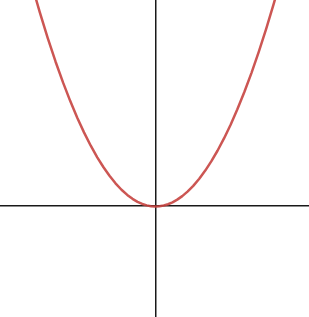
\includegraphics{4.1.2.png}
        \end{center}
        \begin{gather*}
            \lim_{x \to 0+0}\frac{f(x) - f(x_0)}{\Delta x} = \lim_{x\to 0+0} \frac{x^2 - 0}{x - 0} = 0\\
            \lim_{x \to 0-0}\frac{f(-x) - f(x_0)}{\Delta x} = \lim_{x\to 0-0} \frac{x^2 - 0}{-x-0} = 0
        \end{gather*}
        В точке $x = 0$ действительно $f'(x) = 0$.
        \begin{center}
            \textbf{Ч.т.д.}
        \end{center}
    \end{adjustwidth}
    
    \subsubsection*{Теорема 1.1}
    Функция, имеющая конечную производную в точке, непрерывна в этой точке.\par\noindent
    \underline{Доказательство:}
    \begin{adjustwidth}{1.5em}{1.5em}
        Пусть существует $\lim_{x\to x_0} \frac{\Delta y}{\Delta x} = f'$ конечное.
        \[ \frac{\Delta y}{\Delta x} = f' + \varepsilon(\Delta x), \lim_{\Delta x \to 0}\varepsilon(\Delta x) = 0 \]
        \[ \Delta y = f' \Delta x + \varepsilon(\Delta x)\Delta x \]
        \[ \lim_{\Delta x \to 0} \Delta y = \lim_{\Delta x \to 0} (f' \Delta x + \varepsilon(\Delta x)\Delta x) = \lim_{\Delta x \to 0} f'\Delta x + \lim_{\Delta x \to 0} \varepsilon(\Delta x)\Delta x = 0 + 0 = 0 \]
        \begin{center}
            \textbf{Ч.т.д.}
        \end{center}
    \end{adjustwidth}

    \noindent Мгновенная скорость\par\noindent
    Пусть $S = S(t)$ - закон движения в точке.\\
    Рассмотрим $[ t, t + \Delta t ]$: $\Delta S = S(t+\Delta t) - S(t)$ - путь, пройденный за промежуток времени $\Delta t$.\\
    $v_{\text{ср}} = \frac{\Delta S}{\Delta t}$ - средняя скорость.\\
    Мгновенная скорость $v = \lim_{\Delta t \to 0} \frac{\Delta S}{\Delta t} = S'(t)$\\
    $a = \lim_{\Delta t \to 0} \frac{\Delta v}{\Delta t}$ - ускорение.

    \subsection{Геометрический смысл прооизводной}
    \begin{center}
        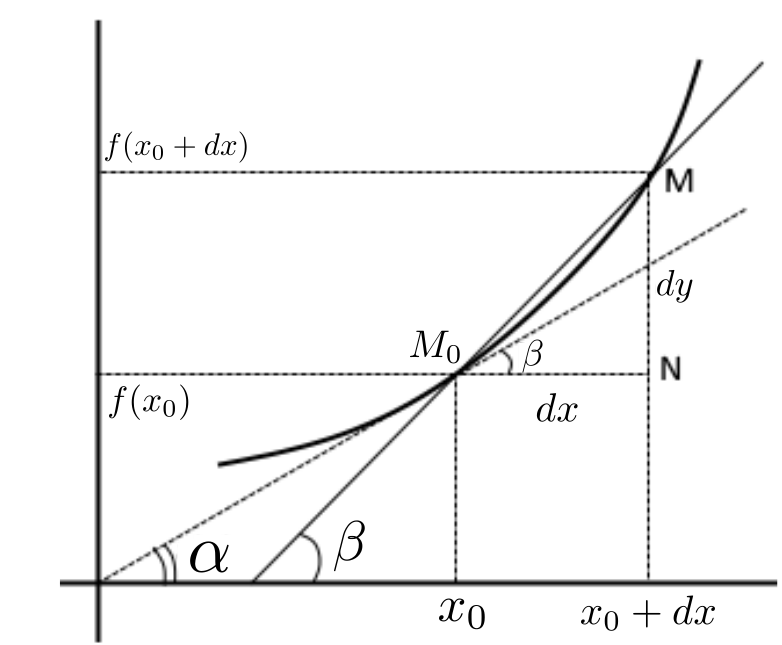
\includegraphics{4.2.1.png}
    \end{center}
    \[ M_0(x_0; f(x_0)) \]
    \[ M(x_0 + \Delta x; f(x_0 + \Delta x)) \]
    Запишем уравнение прямой $M_0M$\\
    \underline{Замечание:} уравнение прямой, проходящей через точки $(x_0; y_0)$ и $(x_1; y_1)$:
    \[ \frac{x - x_0}{x_1 - x_0} = \frac{y - y_0}{y_1 - y_0} \]
    \begin{gather*}
        \frac{x - x_0}{x_0 + \Delta x - x_0} = \frac{y - f(x_0)}{f(x_0 + \Delta x) - f(x_0)}\\
        \frac{x - x_0}{\Delta x} = \frac{y - y_0}{\Delta y}\\
        \Delta y(x - x_0) = \Delta x(y - y_0) \text{ } \big| \text{ } * \Delta x\\
        y - y_0 = \frac{\Delta y}{\Delta x}(x - x_0)\\
        y = \frac{\Delta y}{\Delta x}(x - x_0) + f(x_0) \text{ } \big| \text{ } : M_0M\\
        \text{tg } \angle \beta = \frac{|MN|}{|M_0N|} = \frac{\Delta y}{\Delta x}
    \end{gather*}
    Пусть $\Delta x \to 0$. Тогда точка $M$ будет стремиться к точке $M_0$, а угол $\beta$ к углу $\alpha$.
    \[ \lim_{\Delta x \to 0} \frac{\Delta y}{\Delta x} = f'(x_0) \text{ по определению} \]
    С другой стороны,
    \[ \lim_{\Delta x \to 0} \frac{\Delta y}{\Delta x} = \lim_{\Delta x \to 0} \text{tg } \beta = tg \lim_{\Delta x \to 0} \beta = tg \alpha \]
    Рассмотрим уравнение секущей при $\Delta x \to 0$
    \[ y = f'(x_0)(x - x_0) + f(x_0) \]
    \begin{center}
        - уравнение касательной к графику функции $f(x)$ в точке $x_0$.
    \end{center}

    Допустим $f'(x_0) = \infty$. Тогда рассмотрим уравнение секущей:
    \begin{gather*}
        y = \frac{\Delta y}{\Delta x} (x-x_0) + y_0 \text{ } \big| \text{ } : \frac{\Delta y}{\Delta x}\\
        \frac{y}{\frac{\Delta y}{\Delta x}} = x - x_0 + \frac{y_0}{\frac{\Delta y}{\Delta x}}
    \end{gather*}
    Перейдём к пределу при $\Delta x \to 0$. Тогда уравнение касательной примет вид \underline{$x = x_0$}.\par\noindent
    \underline{Замечание:} если $L_1 \perp L_2$
    \[ \begin{matrix}
        L_1: y = k_1x + b_1\\
        L_2: y = k_2x + b_2
    \end{matrix} \implies k_1k_2 = -1 \]
    Прямая, проходящая через точку $x_0$ перпендикулярно касательной, проведённой в этой точке, называется \underline{нормалью} к графику функции $f(x)$.
    \[ K_\text{н} = -\frac{1}{K_\text{кас}} = -\frac{1}{f'(x_0)} \]
    \[ y = -\frac{1}{f'(x_0)}(x - x_0) + y_0 \]

    \subsection{Производные элементарных функций}
    \begin{enumerate}
        \item $y = \mathbb{C} = const$\\
        $y(x) = \mathbb{C}, y(x + \Delta x) = \mathbb{C}$
        \[ y' = \lim_{\Delta x \to 0}\frac{y(x+ \Delta x) - y(x)}{\Delta x} = \lim_{\Delta x \to 0}\frac{\mathbb{C} - \mathbb{C}}{\Delta x} = 0 \]
        \item $y = \sin x$
        \[ y' = \lim_{\Delta x \to 0} \frac{\sin(x + \Delta x) - \sin x}{\Delta x} = \lim_{\Delta x \to 0}\frac{2\sin \frac{\Delta x}{2} * \cos (x + \frac{\Delta x}{2})}{\frac{\Delta x}{2} * 2} = \cos x \]
        Аналогично доказывается, что $(\cos x)' = - \sin x$
    \end{enumerate}
\end{document}